\chapter{Análisis de resultados}

\section{Análisis de ingeniería}
%El análisis de ingeniería va enfocado a los cambios realizados a lo largo del proyecto, permitiendo seleccionar la opción que mejor se adapte a los requerimientos establecidos, esto en función del diseño, modelado y simulación realizados. 
De manera transversal, la validación en la etapa de diseño a lo largo del proyecto implicó realizar diferentes cambios del mismo, con el fin de adaptarse a los requerimientos establecidos en la metodología utilizada, así como situaciones y condiciones no previstas. Se hace mención de estos cambios por módulo.

\begin{itemize}
    \item \textbf{Módulo Energético}\\
    \begin{itemize}
        \item Se tenía considerado almacenar toda la energía generada por el seguidor. Sin embargo, esta opción resultó demasiado costosa, por lo que se optó por solo almacenar el consumo suficiente que el seguidor requiere, que es del 3\% generado.
        \item Se iban a utilizar los paneles pequeños con los que ya se contaba (de 100 W), sin embargo al realizar los cálculos nos dimos cuenta que con estos no bastaría para obtener la energía eléctrica propuesta en los objetivos, por lo que se optó por solo utilizar los paneles grandes (de 250 W).
        %\item En el diseño eléctrico realizado en Trabajo Terminal I no se contempló ninguna carga en CA, por lo que no se seleccionó ningún inversor. Ahora en Trabajo Terminal II, para la alimentación del motor se utiliza un driver, el cual se alimenta en CA, entrada que se convierte en voltaje de CC.
    \end{itemize}
    \item \textbf{Módulo de Seguimiento Solar}\\
    \begin{itemize}
        \item Debido a que la reducción dada por las cajas reductoras no era suficiente (100:1) para disminuir la velocidad angular de los motores, se optó por diseñar transmisiones mecánicas para cada uno de los ejes de movimiento con mecanismos corona-sinfín de autobloqueo, con reducciones de 48:1. Eso mismo implicó el diseño y selección de chavetas y anillos de retención para fijar las coronas a sus respectivos ejes mecánicos de movimiento.
        \item Se seleccionaron sensores de fin de carrera diferentes a los que se tenían seleccionados en Trabajo Terminal I (LSPS-171008). Esto debido a que no se tenía definida la localización y la manera de activarlos en la estructura mecánica del robot. La forma de activación de estos sensores se muestra en las Figuras \ref{fig:ls1}-\ref{fig:ls3}.
        \begin{figure}[H]
        	\centering
        	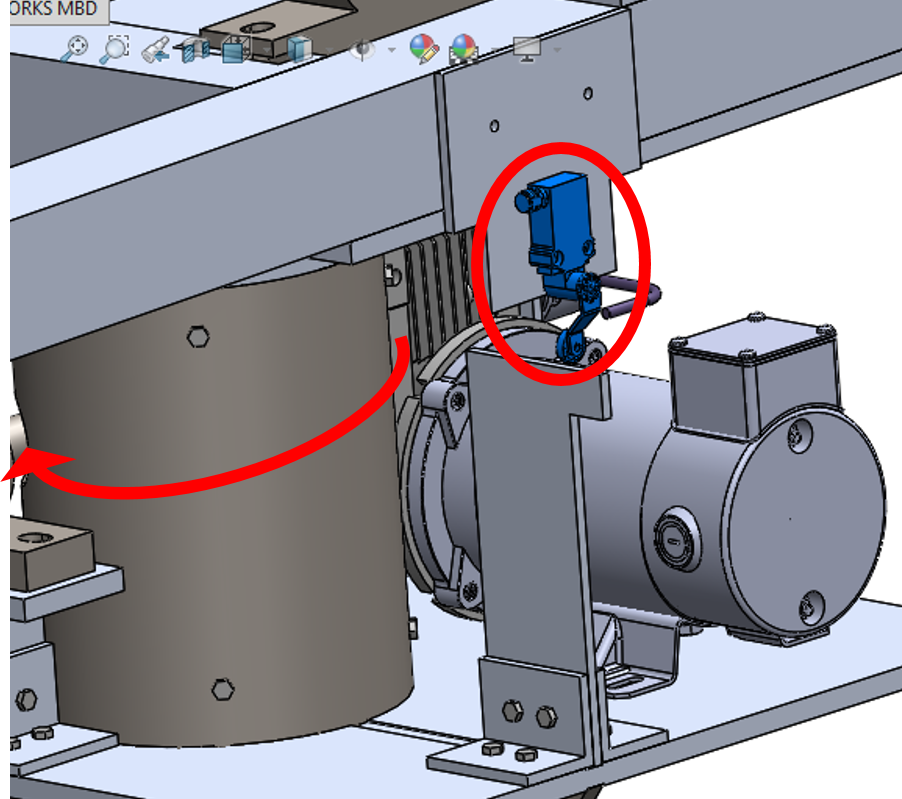
\includegraphics[width=7cm]{imagenes/ls1}
        	\caption{Sensor de fin de carrera \textit{AEM2G4520Z11MR} activado para el movimiento azimutal.}
        	\label{fig:ls1}
        \end{figure}
        \begin{figure}[H]
        	\centering
        	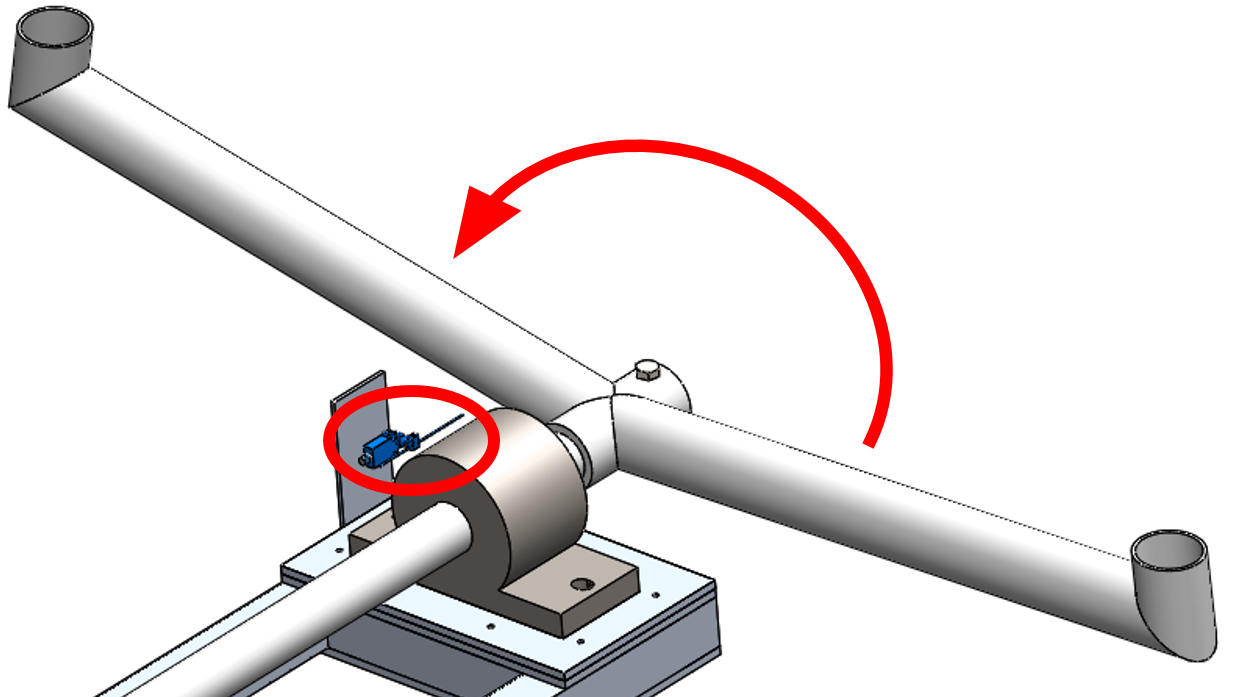
\includegraphics[width=10cm]{imagenes/ls2}
        	\caption{Sensor de fin de carrera \textit{AEM2G7120Z11M} activado para el movimiento de elevación a 90°.}
        	\label{fig:ls2}
        \end{figure}
        \begin{figure}[H]
        	\centering
        	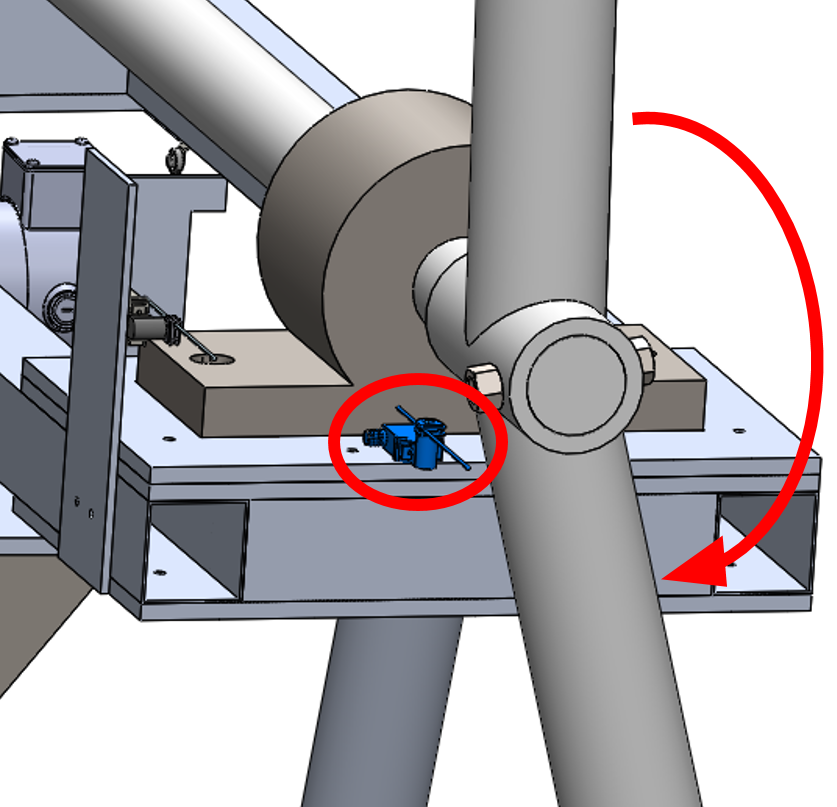
\includegraphics[width=7cm]{imagenes/ls3}
        	\caption{Sensor de fin de carrera \textit{AEM2G7120Z11M} activado para el movimiento de elevación a 0°.}
        	\label{fig:ls3}
        \end{figure}
    \end{itemize}
    \item \textbf{Módulo Estructural}\\
    \begin{itemize}
        \item El diseño de la estructura del colector cambió al aumentar el largo de este en 40 cm. Este cambio se realizó para permitir que el viento pase a través de la estructura, minimizando el esfuerzo producido por el viento. Este cambio se muestra en la Figura \ref{fig:res_col}.
        \begin{figure}[H]
        	\centering
        	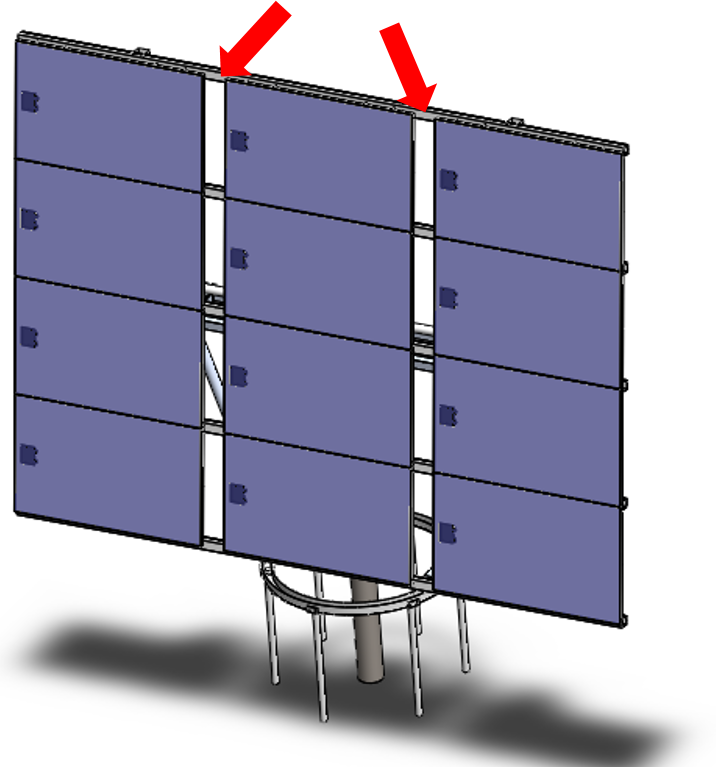
\includegraphics[width=6cm]{imagenes/res_col}
        	\caption{Espacio del colector para permitir el paso del viento.}
        	\label{fig:res_col}
        \end{figure}
        \item Debido a que se presentaba mayor inercia al realizar el movimiento azimutal desde la base, se optó por trasladar este movimiento a la parte superior de la columna principal. Este cambio se ve reflejado en el modelado del robot.
        \item En el diseño preliminar no se consideró una estructura de soporte auxiliar, ya que se pensaba realizar el movimiento de ambos ejes en el punto de unión de la base de elevación con el tubo principal de soporte. Sin embargo, surgió su necesidad como parte del diseño iterativo como solución ante la dificultad de acoplar ambos movimientos en un solo punto sin elevar los costos de manera significativa. Esta estructura tiene dos funciones vitales: 
        \begin{itemize}
            \item Proporcionar estabilidad y soporte a todo el conjunto de elevación y el colector, reduciendo la carga que el tubo principal debe soportar a 1/3 de la original prevista.
        	\item Brindar un espacio exclusivo para generar el movimiento de elevación, gracias a una pista de movimiento especialmente diseñada para esto, permitiendo así que dicho movimiento se refleje en la base de elevación pero que sea soportado, guiado y restringido por la pista ya mencionada.
        \end{itemize}
        
        \item Respecto a los materiales utilizados, se optó por elegir aluminio estructural de la serie 6000 en la mayoría del mecanismo debido al peso y las ventajas que se mostraron sobre el acero. Dichas comparativas se observan en las GUI´s realizadas de la sección de \textit{Estructura del Sistema} del \textit{Módulo Estructural} desde la Figura \ref{fig:GUI_1} hasta la Figura \ref{fig:GUI_3}. Así mismo, como se observa que la elección de dicho material apoya a la necesidad planteada en la Tabla \ref{tabla:needs} con \textit{Facilidad de cambio de piezas/componentes}.
        
        
    \end{itemize}
    \item \textbf{Módulo de Mando Central}\\
    \begin{itemize}
        \item La lógica para seleccionar los modos de operación cambió debido a que fue necesario enfocarlo a programación estructurada, a diferencia de la máquina de estados que se tenía prevista en Trabajo Terminal I.
        \item Para adquirir el PLC se realizó la cotización mostrada en la Figura \ref{fig:plc_cotizacion}, en la cual nos percatamos que costaría el doble de lo previsto en Trabajo Terminal I. Además, por circunstancias que se mencionarán en la sección \textit{Administración de riesgos} fue que se optó por hacer uso de la NUCLEO seleccionada.
        \begin{figure}[H]
        	\centering
        	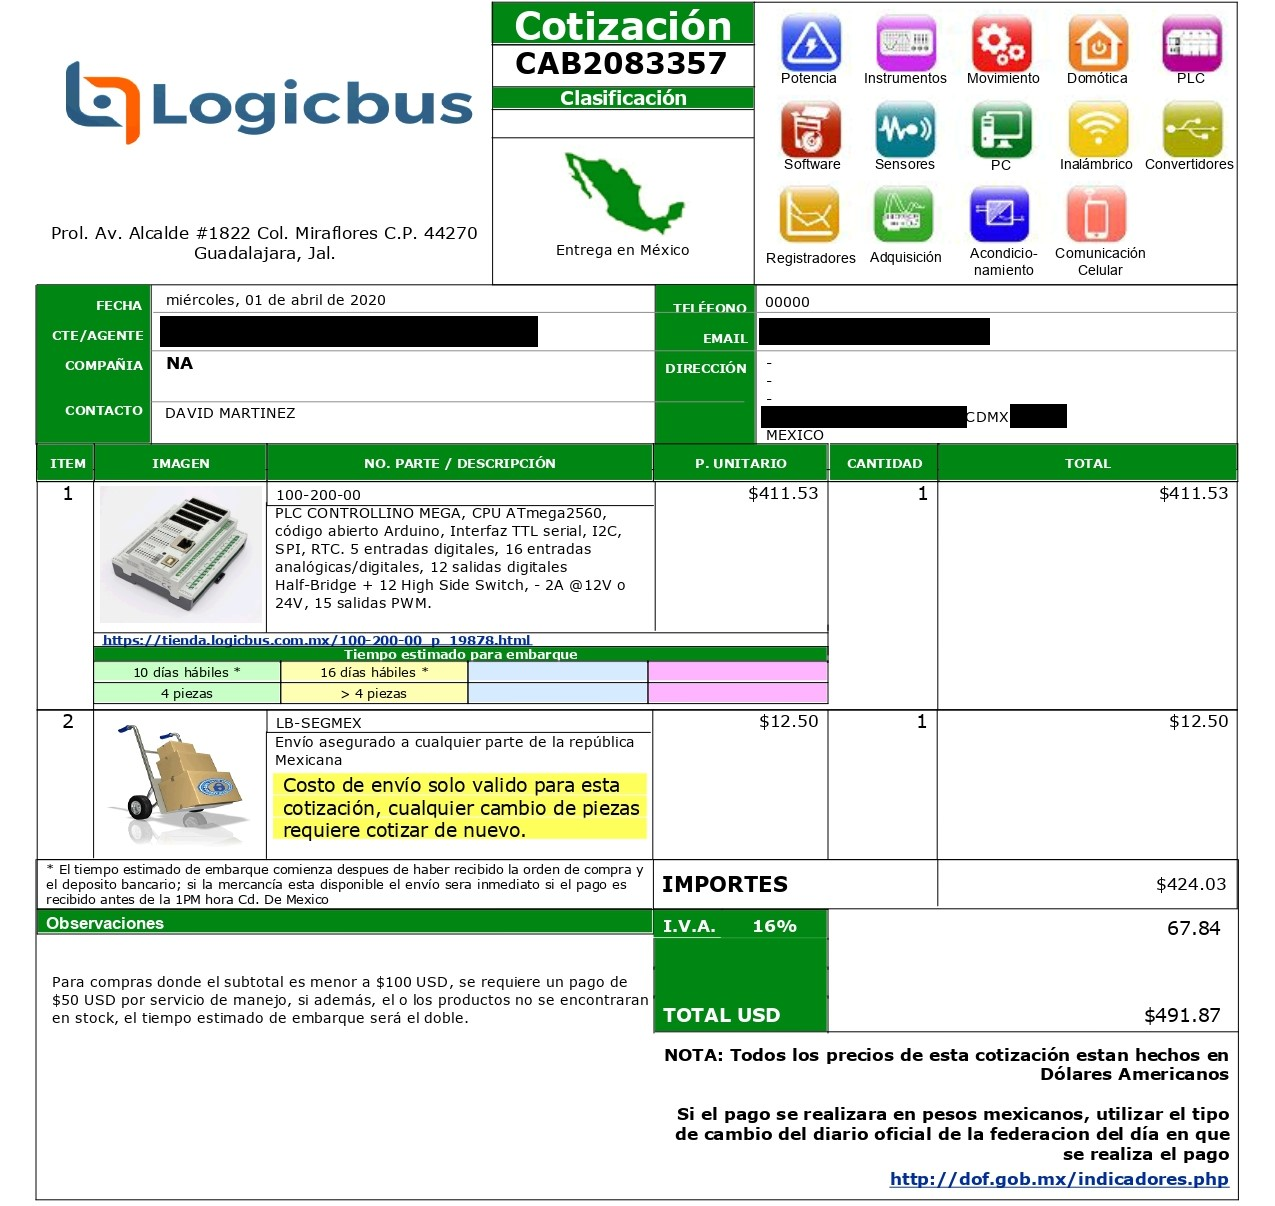
\includegraphics[width=12cm]{imagenes/plc_cotizacion}
        	\caption{Cotización del Controllino MEGA.}
        	\label{fig:plc_cotizacion}
        \end{figure}
    \end{itemize}
    \item \textbf{Módulo de Interfaz}\\
    \item Tomando en cuenta el costo acumulado, se optó por desarrollar la Interfaz en una computadora, lo cual simplificó la red de comunicación entre éste y el dispositivo electrónico de control.
\end{itemize}

\newpage
\section{Análisis de costos}

A continuación, se mostrarán los precios de cada pieza del sistema. Se clasifican por el giro comercial en el que se puede encontrar y se especifica el módulo al que pertenece.\\

En la Tabla \ref{tab:CostoMe} se muestran los precios de las piezas ya cortadas y rectificadas a la medida que se necesita. A dichos materiales se le harán los procesos de manufactura correspondientes a las \textit{Hojas de procesos}. Los precios que se encuentran de color amarillo son los precios de la pieza completamente mecanizada. Dichos precios fueron proporcionados por \cite{Metal}.\\

El material de ferretería (tornillos, tuercas, rondanas, etc), muestra sus precios en la Tabla \ref{tabla:CostoFe} \cite{Toledo}. Los tornillos cuentan con un grado de dureza 8.8. \\

Los rodamientos necesarios, así como las chumaceras y las piezas necesarias para su instalación se localizan en Tabla  \ref{tab:CostoRo}.\\

La lista de materiales y costos de los componentes electrónicos se encuentran en Tabla \ref{tabla:CostoEle}.\\

Para la elaboración de una zapata tipo dado, se muestra el costo de los materiales en Tabla \ref{tab:CostoCi} \cite{Zapatita}. \\

Se encontrará en la Tabla \ref{tab:CostoRu} los precios para la rueda utilizada en el módulo azimutal. \cite{Ruedas}.\\

Considerando los materiales con los que ya se cuenta; se realiza una lista mostrando el total de su precio en Tabla  \ref{tab:CostoYa}.\\

Para hacer una comparativa entre los precios de los metales ya cortados con los precios comerciales, se realiza la cotización del segundo Tabla \ref{tab:CostoComercial}\cite{Metal}.\\
\newpage





%\begin{table}[H]
%	\centering
%	\caption{Estimación de costos}
%	\begin{tabular}{@{}|p{4.5cm}|p{2.5cm}|p{6cm}|}
%		\hline
%		\textbf{Sensor/Dispositivo} & \textbf{Precio (US)} & \textbf{Fuente} \\
%		\hline
%		\textbf{GPS} & \$  25.00  & \url{https://www.u-blox.com/} \\
%		\hline
%		\textbf{Encoder (2)} & \$ 400.00  & \url{https://www.automationdirect.com/} \\
%		\hline
%		\textbf{Fin de carrera} & \$  21.50  & \url{https://www.automationdirect.com/} \\
%		\hline
%		\textbf{Presión} & \$ 150.00  & \url{https://www.mouser.mx/} \\
%		\hline
%		\textbf{Humedad y Temperatura} & \$ 67.00  & \url{https://www.mouser.mx/} \\
%		\hline
%		\textbf{PLC} & \$ 300.00  & \url{https://controllino.es} \\
%		\hline
%		\textbf{Total} & \$ 963.50  &  \\
%		\hline
%	\end{tabular}%
%	\label{tab:costo}%
%\end{table}%

\begin{longtable}{|c|c|c|c|c|c|}
    %\small
	\caption{Cotización de metales cortados y rectificados}\\
	% aquí añadimos el encabezado de la primera hoja.
	\hline
	\rowcolor[rgb]{ 1,  .753,  0} \multicolumn{1}{|p{5.355em}|}{\textbf{Clave}} & \multicolumn{1}{p{4.355em}|}{\textbf{Cantidad}} & \multicolumn{1}{p{10em}|}{\textbf{Costo individual}} & \multicolumn{1}{p{7em}|}{\textbf{Total MXN}} \\
	\hline
	\endfirsthead
	
	% aquí añadimos el encabezado del resto de hojas.
	\hline
	\rowcolor[rgb]{ 1,  .753,  0} \multicolumn{1}{|p{5.355em}|}{\textbf{Clave}} & \multicolumn{1}{p{4.355em}|}{\textbf{Cantidad}} & \multicolumn{1}{p{10em}|}{\textbf{Costo individual}} & \multicolumn{1}{p{7em}|}{\textbf{Total MXN}} \\
	\hline
	\endhead
	
	% aquí añadimos el fondo de todas las hojas, excepto de la última.
	\multicolumn{6}{c}{}
	\endfoot
	
	% aquí añadimos el fondo de la última hoja.
	\endlastfoot
	
	% aquí añadimos el cuerpo de la tabla.

%----
    \hline
    \rowcolor[rgb]{ .867,  .922,  .969} \multicolumn{1}{|l|}{CO\_MC1} & \cellcolor[rgb]{ 1,  1,  1}5 & \multicolumn{1}{r|}{\cellcolor[rgb]{ 1,  1,  1}720} & \cellcolor[rgb]{ 1,  1,  1}3600 \\
    \hline
    \rowcolor[rgb]{ .867,  .922,  .969} \multicolumn{1}{|l|}{CO\_MC2} & \cellcolor[rgb]{ 1,  1,  1}2 & \multicolumn{1}{r|}{\cellcolor[rgb]{ 1,  1,  1}3670} & \cellcolor[rgb]{ 1,  1,  1}7340 \\
    \hline
    \rowcolor[rgb]{ .867,  .922,  .969} \multicolumn{1}{|l|}{CO\_ME1} & \cellcolor[rgb]{ 1,  1,  1}4 & \multicolumn{1}{r|}{\cellcolor[rgb]{ 1,  1,  1}640} & \cellcolor[rgb]{ 1,  1,  1}2560 \\
    \hline
    \rowcolor[rgb]{ .867,  .922,  .969} \multicolumn{1}{|l|}{CO\_ME1} & \cellcolor[rgb]{ 1,  1,  1}8 & \multicolumn{1}{r|}{\cellcolor[rgb]{ 1,  1,  1}640} & \cellcolor[rgb]{ 1,  1,  1}5120 \\
    \hline
    \rowcolor[rgb]{ .867,  .922,  .969} \multicolumn{1}{|l|}{CO\_MC4} & \cellcolor[rgb]{ 1,  1,  1}16 & \multicolumn{1}{r|}{\cellcolor[rgb]{ 1,  1,  1}640} & \cellcolor[rgb]{ 1,  1,  1}10240 \\
    \hline
    \rowcolor[rgb]{ .867,  .922,  .969} \multicolumn{1}{|l|}{CO\_MC3} & \cellcolor[rgb]{ 1,  1,  1}1 & \multicolumn{1}{r|}{\cellcolor[rgb]{ 1,  1,  1}7100} & \cellcolor[rgb]{ 1,  1,  1}7100 \\
    \hline
    \rowcolor[rgb]{ .867,  .922,  .969} \multicolumn{1}{|l|}{CO\_ME2} & \cellcolor[rgb]{ 1,  1,  1}2 & \multicolumn{1}{r|}{\cellcolor[rgb]{ 1,  1,  0}20000} & \cellcolor[rgb]{ 1,  1,  1}40000 \\
    \hline
    \rowcolor[rgb]{ .988,  .894,  .839} \multicolumn{1}{|l|}{AZ\_MC11} & \cellcolor[rgb]{ 1,  1,  1}1 & \multicolumn{1}{r|}{\cellcolor[rgb]{ 1,  1,  1}350} & \cellcolor[rgb]{ 1,  1,  1}350 \\
    \hline
    \rowcolor[rgb]{ .988,  .894,  .839} \multicolumn{1}{|l|}{AZ\_MC12} & \cellcolor[rgb]{ 1,  1,  1}1 & \multicolumn{1}{r|}{\cellcolor[rgb]{ 1,  1,  1}350} & \cellcolor[rgb]{ 1,  1,  1}350 \\
    \hline
    \rowcolor[rgb]{ .988,  .894,  .839} \multicolumn{1}{|l|}{AZ\_MC9} & \cellcolor[rgb]{ 1,  1,  1}1 & \multicolumn{1}{r|}{\cellcolor[rgb]{ 1,  1,  1}850} & \cellcolor[rgb]{ 1,  1,  1}850 \\
    \hline
    \rowcolor[rgb]{ .988,  .894,  .839} \multicolumn{1}{|l|}{AZ\_MC5} & \cellcolor[rgb]{ 1,  1,  1}1 & \multicolumn{1}{r|}{\cellcolor[rgb]{ 1,  1,  1}320} & \cellcolor[rgb]{ 1,  1,  1}320 \\
    \hline
    \rowcolor[rgb]{ .988,  .894,  .839} \multicolumn{1}{|l|}{AZ\_MC6} & \cellcolor[rgb]{ 1,  1,  1}1 & \multicolumn{1}{r|}{\cellcolor[rgb]{ 1,  1,  1}320} & \cellcolor[rgb]{ 1,  1,  1}320 \\
    \hline
    \rowcolor[rgb]{ .988,  .894,  .839} \multicolumn{1}{|l|}{AZ\_MC7} & \cellcolor[rgb]{ 1,  1,  1}1 & \multicolumn{1}{r|}{\cellcolor[rgb]{ 1,  1,  1}330} & \cellcolor[rgb]{ 1,  1,  1}330 \\
    \hline
    \rowcolor[rgb]{ .988,  .894,  .839} \multicolumn{1}{|l|}{AZ\_MC8} & \cellcolor[rgb]{ 1,  1,  1}1 & \multicolumn{1}{r|}{\cellcolor[rgb]{ 1,  1,  1}330} & \cellcolor[rgb]{ 1,  1,  1}330 \\
    \hline
    \rowcolor[rgb]{ .988,  .894,  .839} \multicolumn{1}{|l|}{AZ\_MC3} & \cellcolor[rgb]{ 1,  1,  1}8 & \multicolumn{1}{r|}{\cellcolor[rgb]{ 1,  1,  1}420} & \cellcolor[rgb]{ 1,  1,  1}3360 \\
    \hline
    \rowcolor[rgb]{ .988,  .894,  .839} \multicolumn{1}{|l|}{AZ\_MC4} & \cellcolor[rgb]{ 1,  1,  1}1 & \multicolumn{1}{r|}{\cellcolor[rgb]{ 1,  1,  1}420} & \cellcolor[rgb]{ 1,  1,  1}420 \\
    \hline
    \rowcolor[rgb]{ .988,  .894,  .839} \multicolumn{1}{|l|}{AZ\_MC1} & \cellcolor[rgb]{ 1,  1,  1}2 & \multicolumn{1}{r|}{\cellcolor[rgb]{ 1,  1,  1}350} & \cellcolor[rgb]{ 1,  1,  1}700 \\
    \hline
    \rowcolor[rgb]{ .988,  .894,  .839} \multicolumn{1}{|l|}{AZ\_MC10} & \cellcolor[rgb]{ 1,  1,  1}1 & \multicolumn{1}{r|}{\cellcolor[rgb]{ 1,  1,  1}350} & \cellcolor[rgb]{ 1,  1,  1}350 \\
    \hline
    \rowcolor[rgb]{ .988,  .894,  .839} \multicolumn{1}{|l|}{AZ\_MC2} & \cellcolor[rgb]{ 1,  1,  1}1 & \multicolumn{1}{r|}{\cellcolor[rgb]{ 1,  1,  1}350} & \cellcolor[rgb]{ 1,  1,  1}350 \\
    \hline
    \rowcolor[rgb]{ 1,  .902,  .6} \multicolumn{1}{|l|}{EL\_MC7} & \cellcolor[rgb]{ 1,  1,  1}1 & \multicolumn{1}{r|}{\cellcolor[rgb]{ 1,  1,  1}350} & \cellcolor[rgb]{ 1,  1,  1}350 \\
    \hline
    \rowcolor[rgb]{ 1,  .902,  .6} \multicolumn{1}{|l|}{EL\_MC1} & \cellcolor[rgb]{ 1,  1,  1}1 & \multicolumn{1}{r|}{\cellcolor[rgb]{ 1,  1,  1}490} & \cellcolor[rgb]{ 1,  1,  1}490 \\
    \hline
    \rowcolor[rgb]{ 1,  .902,  .6} \multicolumn{1}{|l|}{EL\_MC2} & \cellcolor[rgb]{ 1,  1,  1}5 & \multicolumn{1}{r|}{\cellcolor[rgb]{ 1,  1,  1}210} & \cellcolor[rgb]{ 1,  1,  1}1050 \\
    \hline
    \rowcolor[rgb]{ 1,  .902,  .6} \multicolumn{1}{|l|}{EL\_MC3} & \cellcolor[rgb]{ 1,  1,  1}1 & \multicolumn{1}{r|}{\cellcolor[rgb]{ 1,  1,  1}890} & \cellcolor[rgb]{ 1,  1,  1}890 \\
    \hline
    \rowcolor[rgb]{ 1,  .902,  .6} \multicolumn{1}{|l|}{EL\_MC4} & \cellcolor[rgb]{ 1,  1,  1}1 & \multicolumn{1}{r|}{\cellcolor[rgb]{ 1,  1,  1}980} & \cellcolor[rgb]{ 1,  1,  1}980 \\
    \hline
    \rowcolor[rgb]{ 1,  .902,  .6} \multicolumn{1}{|l|}{EL\_MC5} & \cellcolor[rgb]{ 1,  1,  1}1 & \multicolumn{1}{r|}{\cellcolor[rgb]{ 1,  1,  1}2180} & \cellcolor[rgb]{ 1,  1,  1}2180 \\
    \hline
    \rowcolor[rgb]{ 1,  .902,  .6} \multicolumn{1}{|l|}{EL\_MC8} & \cellcolor[rgb]{ 1,  1,  1}1 & \multicolumn{1}{r|}{\cellcolor[rgb]{ 1,  1,  1}1970} & \cellcolor[rgb]{ 1,  1,  1}1970 \\
    \hline
    \rowcolor[rgb]{ 1,  .902,  .6} \multicolumn{1}{|l|}{EL\_MC11} & \cellcolor[rgb]{ 1,  1,  1}2 & \multicolumn{1}{r|}{\cellcolor[rgb]{ 1,  1,  1}960} & \cellcolor[rgb]{ 1,  1,  1}1920 \\
    \hline
    \rowcolor[rgb]{ 1,  .902,  .6} \multicolumn{1}{|l|}{EL\_MC14} & \cellcolor[rgb]{ 1,  1,  1}1 & \multicolumn{1}{r|}{\cellcolor[rgb]{ 1,  1,  1}720} & \cellcolor[rgb]{ 1,  1,  1}720 \\
    \hline
    \rowcolor[rgb]{ 1,  .902,  .6} \multicolumn{1}{|l|}{EL\_ME1} & \cellcolor[rgb]{ 1,  1,  1}2 & \multicolumn{1}{r|}{\cellcolor[rgb]{ 1,  1,  1}720} & \cellcolor[rgb]{ 1,  1,  1}1440 \\
    \hline
    \rowcolor[rgb]{ 1,  .902,  .6} \multicolumn{1}{|l|}{EL\_MC13} & \cellcolor[rgb]{ 1,  1,  1}2 & \multicolumn{1}{r|}{\cellcolor[rgb]{ 1,  1,  1}1140} & \cellcolor[rgb]{ 1,  1,  1}2280 \\
    \hline
    \rowcolor[rgb]{ 1,  .902,  .6} \multicolumn{1}{|l|}{EL\_MC9} & \cellcolor[rgb]{ 1,  1,  1}4 & \multicolumn{1}{r|}{\cellcolor[rgb]{ 1,  1,  1}1240} & \cellcolor[rgb]{ 1,  1,  1}4960 \\
    \hline
    \rowcolor[rgb]{ 1,  .902,  .6} \multicolumn{1}{|l|}{EL\_MC6} & \cellcolor[rgb]{ 1,  1,  1}2 & \multicolumn{1}{r|}{\cellcolor[rgb]{ 1,  1,  1}315} & \cellcolor[rgb]{ 1,  1,  1}630 \\
    \hline
    \rowcolor[rgb]{ 1,  .902,  .6} \multicolumn{1}{|l|}{EL\_MC10} & \cellcolor[rgb]{ 1,  1,  1}1 & \multicolumn{1}{r|}{\cellcolor[rgb]{ 1,  1,  1}1420} & \cellcolor[rgb]{ 1,  1,  1}1420 \\
    \hline
    \rowcolor[rgb]{ 1,  .902,  .6} \multicolumn{1}{|l|}{EL\_MC12} & \cellcolor[rgb]{ 1,  1,  1}1 & \multicolumn{1}{r|}{\cellcolor[rgb]{ 1,  1,  1}1420} & \cellcolor[rgb]{ 1,  1,  1}1420 \\
    \hline
    \rowcolor[rgb]{ .776,  .878,  .706} \multicolumn{1}{|l|}{TA\_MC5} & \cellcolor[rgb]{ 1,  1,  1}8 & \multicolumn{1}{r|}{\cellcolor[rgb]{ 1,  1,  1}260} & \cellcolor[rgb]{ 1,  1,  1}2080 \\
    \hline
    \rowcolor[rgb]{ .776,  .878,  .706} \multicolumn{1}{|l|}{TA\_MC1} & \cellcolor[rgb]{ 1,  1,  1}1 & \multicolumn{1}{r|}{\cellcolor[rgb]{ 1,  1,  1}270} & \cellcolor[rgb]{ 1,  1,  1}270 \\
    \hline
    \rowcolor[rgb]{ .776,  .878,  .706} \multicolumn{1}{|l|}{TA\_MC2} & \cellcolor[rgb]{ 1,  1,  1}1 & \multicolumn{1}{r|}{\cellcolor[rgb]{ 1,  1,  1}270} & \cellcolor[rgb]{ 1,  1,  1}270 \\
    \hline
    \rowcolor[rgb]{ .776,  .878,  .706} \multicolumn{1}{|l|}{TA\_MC3} & \cellcolor[rgb]{ 1,  1,  1}1 & \multicolumn{1}{r|}{\cellcolor[rgb]{ 1,  1,  1}270} & \cellcolor[rgb]{ 1,  1,  1}270 \\
    \hline
    \rowcolor[rgb]{ .776,  .878,  .706} \multicolumn{1}{|l|}{TA\_MC4} & \cellcolor[rgb]{ 1,  1,  1}1 & \multicolumn{1}{r|}{\cellcolor[rgb]{ 1,  1,  1}270} & \cellcolor[rgb]{ 1,  1,  1}270 \\
    \hline
    \rowcolor[rgb]{ .776,  .878,  .706} \multicolumn{1}{|l|}{TA\_MC7} & \cellcolor[rgb]{ 1,  1,  1}1 & \multicolumn{1}{r|}{\cellcolor[rgb]{ 1,  1,  1}295} & \cellcolor[rgb]{ 1,  1,  1}295 \\
    \hline
    \rowcolor[rgb]{ .776,  .878,  .706} \multicolumn{1}{|l|}{TA\_MC6} & \cellcolor[rgb]{ 1,  1,  1}1 & \multicolumn{1}{r|}{\cellcolor[rgb]{ 1,  1,  0}7900} & \cellcolor[rgb]{ 1,  1,  1}7900 \\
    \hline
    \rowcolor[rgb]{ .776,  .878,  .706} \multicolumn{1}{|l|}{TA\_ME1} & \cellcolor[rgb]{ 1,  1,  1}1 & \multicolumn{1}{r|}{\cellcolor[rgb]{ 1,  1,  0}3500} & \cellcolor[rgb]{ 1,  1,  1}3500 \\
    \hline
    \rowcolor[rgb]{ .957,  .69,  .518} \multicolumn{1}{|l|}{RO\_MC4} & \cellcolor[rgb]{ 1,  1,  1}2 & \multicolumn{1}{r|}{\cellcolor[rgb]{ 1,  1,  0}5400} & \cellcolor[rgb]{ 1,  1,  1}10800 \\
    \hline
    \rowcolor[rgb]{ .957,  .69,  .518} \multicolumn{1}{|l|}{RO\_MC1} & \cellcolor[rgb]{ 1,  1,  1}6 & \multicolumn{1}{r|}{\cellcolor[rgb]{ 1,  1,  1}795} & \cellcolor[rgb]{ 1,  1,  1}4770 \\
    \hline
    \rowcolor[rgb]{ .957,  .69,  .518} \multicolumn{1}{|l|}{RO\_MC2} & \cellcolor[rgb]{ 1,  1,  1}6 & \multicolumn{1}{r|}{\cellcolor[rgb]{ 1,  1,  1}600} & \cellcolor[rgb]{ 1,  1,  1}3600 \\
    \hline
    \rowcolor[rgb]{ .957,  .69,  .518} \multicolumn{1}{|l|}{RO\_ME1} & \cellcolor[rgb]{ 1,  1,  1}1 & \multicolumn{1}{r|}{\cellcolor[rgb]{ 1,  1,  0}4600} & \cellcolor[rgb]{ 1,  1,  1}4600 \\
    \hline
    \rowcolor[rgb]{ .957,  .69,  .518} \multicolumn{1}{|l|}{RO\_MC3} & \cellcolor[rgb]{ 1,  1,  1}1 & \multicolumn{1}{r|}{\cellcolor[rgb]{ 1,  1,  1}350} & \cellcolor[rgb]{ 1,  1,  1}350 \\
    \hline
    \rowcolor[rgb]{ .675,  .725,  .792} \multicolumn{1}{|l|}{PR\_MC1} & \cellcolor[rgb]{ 1,  1,  1}2 & \multicolumn{1}{r|}{\cellcolor[rgb]{ 1,  1,  1}2800} & \cellcolor[rgb]{ 1,  1,  1}5600 \\
    \hline
    \rowcolor[rgb]{ .675,  .725,  .792} \multicolumn{1}{|l|}{PR\_MC2} & \cellcolor[rgb]{ 1,  1,  1}1 & \multicolumn{1}{r|}{\cellcolor[rgb]{ 1,  1,  0}570} & \cellcolor[rgb]{ 1,  1,  1}570 \\
    \hline
          &       &       &  \\
    \hline
          &       & \textbf{SubTotal} & \textbf{151835} \\
    \hline
          &       & \textbf{IVA 16\%} & \textbf{24293.6} \\
    \hline
          &       & \textbf{Total MXN} & \textbf{ \$ 176,128.60 } \\
    \hline
    % esta línea es importante para que deje un espacio entre la tabla y el nombre de la tabla.
  \label{tab:CostoMe}%
\end{longtable}



\begin{landscape}
%-----------------
\begin{longtable}{|c|c|c|c|c|c|c|}
    %\small
	\caption{Cotización de material de ferretería}\\
	% aquí añadimos el encabezado de la primera hoja.
	
	\hline
	%\rowcolor[rgb]{ 1,  .753,  0}
\multicolumn{1}{|p{7.5em}|}{\cellcolor[rgb]{ 1,  .753,  0}{\textbf{Modulo}}} & \multicolumn{1}{p{8.5em}|}{\cellcolor[rgb]{ 1,  .753,  0}{\textbf{Tipo}}} & \multicolumn{1}{p{5.5em}|}{\cellcolor[rgb]{ 1,  .753,  0}{\textbf{Cabeza}}} & \multicolumn{1}{p{8.5em}|}{\cellcolor[rgb]{ 1,  .753,  0}{\textbf{Especificaciones}}} & \multicolumn{1}{p{5em}|}{\cellcolor[rgb]{ 1,  .753,  0}{\textbf{Cantidad}}} & \multicolumn{1}{p{9em}|}{\cellcolor[rgb]{ 1,  .753,  0}{\textbf{Costo Individual}}} & \multicolumn{1}{p{6.5em}|}{\cellcolor[rgb]{ 1,  .753,  0}{\textbf{Total MXN}}} \\
	\hline
	\endfirsthead
	
	% aquí añadimos el encabezado del resto de hojas.
	\hline
%\rowcolor[rgb]{ 1,  .753,  0}
\multicolumn{1}{|p{7.5em}|}{\cellcolor[rgb]{ 1,  .753,  0}{\textbf{Modulo}}} & \multicolumn{1}{p{8.5em}|}{\cellcolor[rgb]{ 1,  .753,  0}{\textbf{Tipo}}} & \multicolumn{1}{p{5.5em}|}{\cellcolor[rgb]{ 1,  .753,  0}{\textbf{Cabeza}}} & \multicolumn{1}{p{8.5em}|}{\cellcolor[rgb]{ 1,  .753,  0}{\textbf{Especificaciones}}} & \multicolumn{1}{p{5em}|}{\cellcolor[rgb]{ 1,  .753,  0}{\textbf{Cantidad}}} & \multicolumn{1}{p{9em}|}{\cellcolor[rgb]{ 1,  .753,  0}{\textbf{Costo Individual}}} & \multicolumn{1}{p{6.5em}|}{\cellcolor[rgb]{ 1,  .753,  0}{\textbf{Total MXN}}} \\
	\hline
	\endhead
	
	% aquí añadimos el fondo de todas las hojas, excepto de la última.
	\multicolumn{6}{c}{}
	\endfoot
	
	% aquí añadimos el fondo de la última hoja.
	\endlastfoot
	
	% aquí añadimos el cuerpo de la tabla.
% Table generated by Excel2LaTeX from sheet 'Ferreteria precios'

    \hline
    \rowcolor[rgb]{ .988,  .894,  .839} \multicolumn{1}{|l|}{Azimutal} & \multicolumn{1}{l|}{\cellcolor[rgb]{ 1,  1,  0}Tornillo} & \multicolumn{1}{l|}{\cellcolor[rgb]{ 1,  .851,  .4}Hexagonal} & \multicolumn{1}{c|}{\cellcolor[rgb]{ 1,  1,  1}DIN 931: M6x25} & \cellcolor[rgb]{ 1,  1,  1}24 & \multicolumn{1}{r|}{\cellcolor[rgb]{ 1,  1,  1}2.19} & \cellcolor[rgb]{ 1,  1,  1}52.56 \\
    \hline
    \rowcolor[rgb]{ .988,  .894,  .839} \multicolumn{1}{|l|}{Azimutal} & \multicolumn{1}{l|}{\cellcolor[rgb]{ .573,  .816,  .314}Tuerca} & \multicolumn{1}{l|}{\cellcolor[rgb]{ 1,  .851,  .4}Hexagonal} & \multicolumn{1}{l|}{\cellcolor[rgb]{ 1,  1,  1}DIN 934: M6} & \cellcolor[rgb]{ 1,  1,  1}24 & \multicolumn{1}{r|}{\cellcolor[rgb]{ 1,  1,  1}0.62} & \cellcolor[rgb]{ 1,  1,  1}14.88 \\
    \hline
    \rowcolor[rgb]{ .988,  .894,  .839} \multicolumn{1}{|l|}{Azimutal} & \multicolumn{1}{l|}{\cellcolor[rgb]{ 1,  .753,  0}Rondana Plana} & \multicolumn{1}{l|}{\cellcolor[rgb]{ 1,  1,  1}NA} & \multicolumn{1}{l|}{\cellcolor[rgb]{ 1,  1,  1}DIN 9021: M16} & \cellcolor[rgb]{ 1,  1,  1}2 & \multicolumn{1}{r|}{\cellcolor[rgb]{ 1,  1,  1}3.36} & \cellcolor[rgb]{ 1,  1,  1}6.72 \\
    \hline
    \rowcolor[rgb]{ .988,  .894,  .839} \multicolumn{1}{|l|}{Azimutal} & \multicolumn{1}{l|}{\cellcolor[rgb]{ 0,  .69,  .314}Rondana Presion} & \multicolumn{1}{l|}{\cellcolor[rgb]{ 1,  1,  1}NA} & \multicolumn{1}{l|}{\cellcolor[rgb]{ 1,  1,  1}DIN 127-B: M16} & \cellcolor[rgb]{ 1,  1,  1}2 & \multicolumn{1}{r|}{\cellcolor[rgb]{ 1,  1,  1}3.209} & \cellcolor[rgb]{ 1,  1,  1}6.418 \\
    \hline
    \rowcolor[rgb]{ .988,  .894,  .839} \multicolumn{1}{|l|}{Azimutal} & \multicolumn{1}{l|}{\cellcolor[rgb]{ 1,  1,  0}Tornillo} & \multicolumn{1}{l|}{\cellcolor[rgb]{ 1,  1,  1}Hexagonal} & \multicolumn{1}{l|}{\cellcolor[rgb]{ 1,  1,  1}DIN 933: M8x80} & \cellcolor[rgb]{ 1,  1,  1}4 & \multicolumn{1}{r|}{\cellcolor[rgb]{ 1,  1,  1}12.35} & \cellcolor[rgb]{ 1,  1,  1}49.4 \\
    \hline
    \rowcolor[rgb]{ .988,  .894,  .839} \multicolumn{1}{|l|}{Azimutal } & \multicolumn{1}{l|}{\cellcolor[rgb]{ .573,  .816,  .314}Tuerca} & \multicolumn{1}{l|}{\cellcolor[rgb]{ 1,  1,  1}Hexagonal} & \multicolumn{1}{l|}{\cellcolor[rgb]{ 1,  1,  1}DIN 934: M8} & \cellcolor[rgb]{ 1,  1,  1}8 & \multicolumn{1}{r|}{\cellcolor[rgb]{ 1,  1,  1}1.92} & \cellcolor[rgb]{ 1,  1,  1}15.36 \\
    \hline
    \rowcolor[rgb]{ .988,  .894,  .839} \multicolumn{1}{|l|}{Azimutal } & \multicolumn{1}{l|}{\cellcolor[rgb]{ 1,  0,  0}\textbf{Tuerca Unión}} & \multicolumn{1}{l|}{\cellcolor[rgb]{ 1,  1,  1}Hexagonal} & \multicolumn{1}{l|}{\cellcolor[rgb]{ 1,  1,  1}NA} & \cellcolor[rgb]{ 1,  1,  1}4 & \multicolumn{1}{r|}{\cellcolor[rgb]{ 1,  1,  1}116.16} & \cellcolor[rgb]{ 1,  1,  1}464.64 \\
    \hline
    \rowcolor[rgb]{ .867,  .922,  .969} \multicolumn{1}{|l|}{Colector} & \multicolumn{1}{l|}{\cellcolor[rgb]{ 1,  1,  0}Tornillo} & \multicolumn{1}{l|}{\cellcolor[rgb]{ 1,  .851,  .4}Hexagonal} & \multicolumn{1}{l|}{\cellcolor[rgb]{ 1,  1,  1}DIN 931: M20x120 } & \cellcolor[rgb]{ 1,  1,  1}2 & \multicolumn{1}{r|}{\cellcolor[rgb]{ 1,  1,  1}109.99} & \cellcolor[rgb]{ 1,  1,  1}219.98 \\
   \hline
    \rowcolor[rgb]{ .867,  .922,  .969} \multicolumn{1}{|l|}{Colector} & \multicolumn{1}{l|}{\cellcolor[rgb]{ .573,  .816,  .314}Tuerca} & \multicolumn{1}{l|}{\cellcolor[rgb]{ 1,  .851,  .4}Hexagonal} & \multicolumn{1}{l|}{\cellcolor[rgb]{ 1,  1,  1}DIN 934: M20} & \cellcolor[rgb]{ 1,  1,  1}2 & \multicolumn{1}{r|}{\cellcolor[rgb]{ 1,  1,  1}19.05} & \cellcolor[rgb]{ 1,  1,  1}38.1 \\
    \hline
    \rowcolor[rgb]{ .867,  .922,  .969} \multicolumn{1}{|l|}{Colector} & \multicolumn{1}{l|}{\cellcolor[rgb]{ 1,  1,  0}Tornillo} & \multicolumn{1}{l|}{\cellcolor[rgb]{ 1,  .851,  .4}Hexagonal} & \multicolumn{1}{l|}{\cellcolor[rgb]{ 1,  1,  1}DIN 931: M12x130 } & \cellcolor[rgb]{ 1,  1,  1}8 & \multicolumn{1}{r|}{\cellcolor[rgb]{ 1,  1,  1}42.77} & \cellcolor[rgb]{ 1,  1,  1}342.16 \\
    \hline
    \rowcolor[rgb]{ .867,  .922,  .969} \multicolumn{1}{|l|}{Colector} & \multicolumn{1}{l|}{\cellcolor[rgb]{ .573,  .816,  .314}Tuerca} & \multicolumn{1}{l|}{\cellcolor[rgb]{ 1,  .851,  .4}Hexagonal} & \multicolumn{1}{l|}{\cellcolor[rgb]{ 1,  1,  1}DIN 934: M12} & \cellcolor[rgb]{ 1,  1,  1}8 & \multicolumn{1}{r|}{\cellcolor[rgb]{ 1,  1,  1}4.54} & \cellcolor[rgb]{ 1,  1,  1}36.32 \\
    \hline
    \rowcolor[rgb]{ .867,  .922,  .969} \multicolumn{1}{|l|}{Colector} & \multicolumn{1}{l|}{\cellcolor[rgb]{ 1,  1,  0}Tornillo} & \multicolumn{1}{l|}{\cellcolor[rgb]{ 1,  .851,  .4}Hexagonal} & \multicolumn{1}{l|}{\cellcolor[rgb]{ 1,  1,  1}DIN 931: M10x110 } & \cellcolor[rgb]{ 1,  1,  1}64 & \multicolumn{1}{r|}{\cellcolor[rgb]{ 1,  1,  1}26.22} & \cellcolor[rgb]{ 1,  1,  1}1678.08 \\
    \hline
    \rowcolor[rgb]{ .867,  .922,  .969} \multicolumn{1}{|l|}{Colector} & \multicolumn{1}{l|}{\cellcolor[rgb]{ .573,  .816,  .314}Tuerca} & \multicolumn{1}{l|}{\cellcolor[rgb]{ 1,  .851,  .4}Hexagonal} & \multicolumn{1}{l|}{\cellcolor[rgb]{ 1,  1,  1}DIN 934: M10 } & \cellcolor[rgb]{ 1,  1,  1}64 & \multicolumn{1}{r|}{\cellcolor[rgb]{ 1,  1,  1}3.2} & \cellcolor[rgb]{ 1,  1,  1}204.8 \\
    \hline
    \rowcolor[rgb]{ 1,  .902,  .6} \multicolumn{1}{|l|}{Elevación} & \multicolumn{1}{l|}{\cellcolor[rgb]{ 1,  1,  0}Tornillo} & \multicolumn{1}{l|}{\cellcolor[rgb]{ 1,  .851,  .4}Hexagonal} & \multicolumn{1}{l|}{\cellcolor[rgb]{ 1,  1,  1}DIN 931: M6x25 } & \cellcolor[rgb]{ 1,  1,  1}8 & \multicolumn{1}{r|}{\cellcolor[rgb]{ 1,  1,  1}2.19} & \cellcolor[rgb]{ 1,  1,  1}17.52 \\
    \hline
    \rowcolor[rgb]{ 1,  .902,  .6} \multicolumn{1}{|l|}{Elevación} & \multicolumn{1}{l|}{\cellcolor[rgb]{ .573,  .816,  .314}Tuerca} & \multicolumn{1}{l|}{\cellcolor[rgb]{ 1,  .851,  .4}Hexagonal} & \multicolumn{1}{l|}{\cellcolor[rgb]{ 1,  1,  1}DIN 934: M6 } & \cellcolor[rgb]{ 1,  1,  1}8 & \multicolumn{1}{r|}{\cellcolor[rgb]{ 1,  1,  1}0.62} & \cellcolor[rgb]{ 1,  1,  1}4.96 \\
    \hline
    \rowcolor[rgb]{ 1,  .902,  .6} \multicolumn{1}{|l|}{Elevación} & \multicolumn{1}{l|}{\cellcolor[rgb]{ 1,  1,  0}Tornillo} & \multicolumn{1}{l|}{\cellcolor[rgb]{ 1,  1,  1}Hexagonal} & \multicolumn{1}{l|}{\cellcolor[rgb]{ 1,  1,  1}DIN 933: M8x80} & \cellcolor[rgb]{ 1,  1,  1}4 & \multicolumn{1}{r|}{\cellcolor[rgb]{ 1,  1,  1}12.35} & \cellcolor[rgb]{ 1,  1,  1}49.4 \\
    \hline
    \rowcolor[rgb]{ 1,  .902,  .6} \multicolumn{1}{|l|}{Elevación} & \multicolumn{1}{l|}{\cellcolor[rgb]{ .573,  .816,  .314}Tuerca} & \multicolumn{1}{l|}{\cellcolor[rgb]{ 1,  1,  1}Hexagonal} & \multicolumn{1}{l|}{\cellcolor[rgb]{ 1,  1,  1}DIN 934: M8} & \cellcolor[rgb]{ 1,  1,  1}4 & \multicolumn{1}{r|}{\cellcolor[rgb]{ 1,  1,  1}1.92} & \cellcolor[rgb]{ 1,  1,  1}7.68 \\
    \hline
    \rowcolor[rgb]{ 1,  .902,  .6} \multicolumn{1}{|l|}{Elevación} & \multicolumn{1}{l|}{\cellcolor[rgb]{ 1,  0,  0}\textbf{Tuerca Unión}} & \multicolumn{1}{l|}{\cellcolor[rgb]{ 1,  1,  1}Hexagonal} & \multicolumn{1}{l|}{\cellcolor[rgb]{ 1,  1,  1}NA} & \cellcolor[rgb]{ 1,  1,  1}4 & \multicolumn{1}{r|}{\cellcolor[rgb]{ 1,  1,  1}116.16} & \cellcolor[rgb]{ 1,  1,  1}464.64 \\
    \hline
    \rowcolor[rgb]{ .957,  .69,  .518} \multicolumn{1}{|l|}{Rolado} & \multicolumn{1}{l|}{\cellcolor[rgb]{ 1,  1,  0}Tornillo} & \multicolumn{1}{l|}{\cellcolor[rgb]{ .741,  .843,  .933}Plana Allen} & \multicolumn{1}{l|}{\cellcolor[rgb]{ 1,  1,  1}DIN 7991: M10x30 } & \cellcolor[rgb]{ 1,  1,  1}24 & \multicolumn{1}{r|}{\cellcolor[rgb]{ 1,  1,  1}11.12} & \cellcolor[rgb]{ 1,  1,  1}266.88 \\
    \hline
    \rowcolor[rgb]{ .957,  .69,  .518} \multicolumn{1}{|l|}{Rolado} & \multicolumn{1}{l|}{\cellcolor[rgb]{ .573,  .816,  .314}Tuerca} & \multicolumn{1}{l|}{\cellcolor[rgb]{ 1,  .851,  .4}Hexagonal} & \multicolumn{1}{l|}{\cellcolor[rgb]{ 1,  1,  1}DIN 934: M10} & \cellcolor[rgb]{ 1,  1,  1}24 & \multicolumn{1}{r|}{\cellcolor[rgb]{ 1,  1,  1}3.81} & \cellcolor[rgb]{ 1,  1,  1}91.44 \\
    \hline
    \rowcolor[rgb]{ .957,  .69,  .518} \multicolumn{1}{|l|}{Rolado} & \multicolumn{1}{l|}{\cellcolor[rgb]{ 1,  .753,  0}Rondana Plana} & \multicolumn{1}{l|}{\cellcolor[rgb]{ 1,  1,  1}NA} & \multicolumn{1}{l|}{\cellcolor[rgb]{ 1,  1,  1}DIN 9021: M10} & \cellcolor[rgb]{ 1,  1,  1}12 & \multicolumn{1}{r|}{\cellcolor[rgb]{ 1,  1,  1}1.27} & \cellcolor[rgb]{ 1,  1,  1}15.24 \\
    \hline
    \rowcolor[rgb]{ .957,  .69,  .518} \multicolumn{1}{|l|}{Rolado} & \multicolumn{1}{l|}{\cellcolor[rgb]{ 0,  .69,  .314}Rondana Presión} & \multicolumn{1}{l|}{\cellcolor[rgb]{ 1,  1,  1}NA} & \multicolumn{1}{l|}{\cellcolor[rgb]{ 1,  1,  1}DIN 127-B: M10} & \cellcolor[rgb]{ 1,  1,  1}12 & \multicolumn{1}{r|}{\cellcolor[rgb]{ 1,  1,  1}0.995} & \cellcolor[rgb]{ 1,  1,  1}11.94 \\
    \hline
    \rowcolor[rgb]{ .776,  .878,  .706} \multicolumn{1}{|l|}{Tallo} & \multicolumn{1}{l|}{\cellcolor[rgb]{ .573,  .816,  .314}Tuerca} & \multicolumn{1}{l|}{\cellcolor[rgb]{ 1,  .851,  .4}Hexagonal} & \multicolumn{1}{l|}{\cellcolor[rgb]{ 1,  1,  1}DIN 934: M8  } & \cellcolor[rgb]{ 1,  1,  1}4 & \multicolumn{1}{r|}{\cellcolor[rgb]{ 1,  1,  1}1.92} & \cellcolor[rgb]{ 1,  1,  1}7.68 \\
    \hline
    \rowcolor[rgb]{ .776,  .878,  .706} \multicolumn{1}{|l|}{Tallo} & \multicolumn{1}{l|}{\cellcolor[rgb]{ 1,  1,  0}Tornillo} & \multicolumn{1}{l|}{\cellcolor[rgb]{ 1,  .851,  .4}Hexagonal} & \multicolumn{1}{l|}{\cellcolor[rgb]{ 1,  1,  1}DIN 931: M6x25 } & \cellcolor[rgb]{ 1,  1,  1}12 & \multicolumn{1}{r|}{\cellcolor[rgb]{ 1,  1,  1}2.19} & \cellcolor[rgb]{ 1,  1,  1}26.28 \\
    \hline
    \rowcolor[rgb]{ .776,  .878,  .706} \multicolumn{1}{|l|}{Tallo} & \multicolumn{1}{l|}{\cellcolor[rgb]{ .573,  .816,  .314}Tuerca} & \multicolumn{1}{l|}{\cellcolor[rgb]{ 1,  .851,  .4}Hexagonal} & \multicolumn{1}{l|}{\cellcolor[rgb]{ 1,  1,  1}DIN 934: M6 } & \cellcolor[rgb]{ 1,  1,  1}12 & \multicolumn{1}{r|}{\cellcolor[rgb]{ 1,  1,  1}0.62} & \cellcolor[rgb]{ 1,  1,  1}7.44 \\
    \hline
    \rowcolor[rgb]{ .776,  .878,  .706} \multicolumn{1}{|l|}{Tallo} & \multicolumn{1}{l|}{\cellcolor[rgb]{ 1,  1,  0}Tornillo} & \multicolumn{1}{l|}{\cellcolor[rgb]{ 1,  .851,  .4}Hexagonal} & \multicolumn{1}{l|}{\cellcolor[rgb]{ 1,  1,  1}DIN 931: M16x40 } & \cellcolor[rgb]{ 1,  1,  1}4 & \multicolumn{1}{r|}{\cellcolor[rgb]{ 1,  1,  1}26.22} & \cellcolor[rgb]{ 1,  1,  1}104.88 \\
    \hline
    \rowcolor[rgb]{ .776,  .878,  .706} \multicolumn{1}{|l|}{Tallo} & \multicolumn{1}{l|}{\cellcolor[rgb]{ .573,  .816,  .314}Tuerca} & \multicolumn{1}{l|}{\cellcolor[rgb]{ 1,  .851,  .4}Hexagonal} & \multicolumn{1}{l|}{\cellcolor[rgb]{ 1,  1,  1}DIN 934: M16 } & \cellcolor[rgb]{ 1,  1,  1}4 & \multicolumn{1}{r|}{\cellcolor[rgb]{ 1,  1,  1}8.91} & \cellcolor[rgb]{ 1,  1,  1}35.64 \\
    \hline
    \rowcolor[rgb]{ .776,  .878,  .706} \multicolumn{1}{|l|}{Tallo} & \multicolumn{1}{l|}{\cellcolor[rgb]{ 1,  1,  0}Tornillo} & \multicolumn{1}{l|}{\cellcolor[rgb]{ 1,  .851,  .4}Hexagonal} & \multicolumn{1}{l|}{\cellcolor[rgb]{ 1,  1,  1}DIN 931: M12x80 } & \cellcolor[rgb]{ 1,  1,  1}1 & \multicolumn{1}{r|}{\cellcolor[rgb]{ 1,  1,  1}28.67} & \cellcolor[rgb]{ 1,  1,  1}28.67 \\
    \hline
    \rowcolor[rgb]{ .776,  .878,  .706} \multicolumn{1}{|l|}{Tallo} & \multicolumn{1}{l|}{\cellcolor[rgb]{ .573,  .816,  .314}Tuerca} & \multicolumn{1}{l|}{\cellcolor[rgb]{ 1,  .851,  .4}Hexagonal} & \multicolumn{1}{l|}{\cellcolor[rgb]{ 1,  1,  1}DIN 934: M12 } & \cellcolor[rgb]{ 1,  1,  1}1 & \multicolumn{1}{r|}{\cellcolor[rgb]{ 1,  1,  1}4.32} & \cellcolor[rgb]{ 1,  1,  1}4.32 \\
    \hline
    \rowcolor[rgb]{ .776,  .878,  .706} \multicolumn{1}{|l|}{Tallo} & \multicolumn{1}{l|}{\cellcolor[rgb]{ 0,  .69,  .941}Esparrago} & \multicolumn{1}{l|}{\cellcolor[rgb]{ 1,  1,  1}NA} & \multicolumn{1}{l|}{\cellcolor[rgb]{ 1,  1,  1}DIN 975: M8x1000} & \cellcolor[rgb]{ 1,  1,  1}2 & \multicolumn{1}{r|}{\cellcolor[rgb]{ 1,  1,  1}240} & \cellcolor[rgb]{ 1,  1,  1}480 \\
    \hline
    \rowcolor[rgb]{ .776,  .878,  .706} \multicolumn{1}{|l|}{Tallo} & \multicolumn{1}{l|}{\cellcolor[rgb]{ 0,  .69,  .941}Esparrago} & \multicolumn{1}{l|}{\cellcolor[rgb]{ 1,  1,  1}NA} & \multicolumn{1}{l|}{\cellcolor[rgb]{ 1,  1,  1}DIN 975: M8x300} & \cellcolor[rgb]{ 1,  1,  1}4 & \multicolumn{1}{r|}{\cellcolor[rgb]{ 1,  1,  1}240} & \cellcolor[rgb]{ 1,  1,  1}960 \\
    \hline
    \rowcolor[rgb]{ .776,  .878,  .706} \multicolumn{1}{|l|}{Tallo} & \multicolumn{1}{l|}{\cellcolor[rgb]{ 0,  .69,  .941}Anillo de retención} & \multicolumn{1}{l|}{\cellcolor[rgb]{ 1,  1,  1}NA} & \multicolumn{1}{l|}{\cellcolor[rgb]{ 1,  1,  1}SH-200} & \cellcolor[rgb]{ 1,  1,  1}2 & \multicolumn{1}{r|}{\cellcolor[rgb]{ 1,  1,  1}14} & \cellcolor[rgb]{ 1,  1,  1}28 \\
    \hline
    \rowcolor[rgb]{ .867,  .922,  .969} \multicolumn{1}{|l|}{Colector} & \multicolumn{1}{l|}{\cellcolor[rgb]{ 1,  1,  0}Tornillo} & \multicolumn{1}{l|}{\cellcolor[rgb]{ 1,  .851,  .4}Hexagonal} & \multicolumn{1}{l|}{\cellcolor[rgb]{ 1,  1,  1}DIN 933: M8x60} & \cellcolor[rgb]{ 1,  1,  1}96 & \multicolumn{1}{r|}{\cellcolor[rgb]{ 1,  1,  1}9.89} & \cellcolor[rgb]{ 1,  1,  1}949.44 \\
    \hline
    \rowcolor[rgb]{ .867,  .922,  .969} \multicolumn{1}{|l|}{Colector} & \multicolumn{1}{l|}{\cellcolor[rgb]{ .573,  .816,  .314}Tuerca} & \multicolumn{1}{l|}{\cellcolor[rgb]{ 1,  .851,  .4}Hexagonal} & \multicolumn{1}{l|}{\cellcolor[rgb]{ 1,  1,  1}DIN 934: M8   } & \cellcolor[rgb]{ 1,  1,  1}96 & \multicolumn{1}{r|}{\cellcolor[rgb]{ 1,  1,  1}1.92} & \cellcolor[rgb]{ 1,  1,  1}184.32 \\
    \hline
    \rowcolor[rgb]{ .867,  .922,  .969} \multicolumn{1}{|l|}{Colector} & \multicolumn{1}{l|}{\cellcolor[rgb]{ 1,  .753,  0}Rondana Plana} & \multicolumn{1}{l|}{\cellcolor[rgb]{ 1,  1,  1}NA} & \multicolumn{1}{l|}{\cellcolor[rgb]{ 1,  1,  1}DIN 9021: M8} & \cellcolor[rgb]{ 1,  1,  1}96 & \multicolumn{1}{r|}{\cellcolor[rgb]{ 1,  1,  1}0.71} & \cellcolor[rgb]{ 1,  1,  1}68.16 \\
    \hline
    \rowcolor[rgb]{ .867,  .922,  .969} \multicolumn{1}{|l|}{Colector} & \multicolumn{1}{l|}{\cellcolor[rgb]{ 0,  .69,  .314}Rondana Presión} & \multicolumn{1}{l|}{\cellcolor[rgb]{ 1,  1,  1}NA} & \multicolumn{1}{l|}{\cellcolor[rgb]{ 1,  1,  1}DIN 127-B: M8} & \cellcolor[rgb]{ 1,  1,  1}96 & \multicolumn{1}{r|}{\cellcolor[rgb]{ 1,  1,  1}0.679} & \cellcolor[rgb]{ 1,  1,  1}65.184 \\
    \hline
    \rowcolor[rgb]{ .867,  .922,  .969} \multicolumn{1}{|l|}{Colector} & \multicolumn{1}{l|}{\cellcolor[rgb]{ 1,  .753,  0}Rondana Plana} & \multicolumn{1}{l|}{\cellcolor[rgb]{ 1,  1,  1}NA} & \multicolumn{1}{l|}{\cellcolor[rgb]{ 1,  1,  1}DIN 9021: M12} & \cellcolor[rgb]{ 1,  1,  1}8 & \multicolumn{1}{r|}{\cellcolor[rgb]{ 1,  1,  1}2.26} & \cellcolor[rgb]{ 1,  1,  1}18.08 \\
    \hline
    \rowcolor[rgb]{ .867,  .922,  .969} \multicolumn{1}{|l|}{Colector} & \multicolumn{1}{l|}{\cellcolor[rgb]{ 0,  .69,  .314}Rondana Presión} & \multicolumn{1}{l|}{\cellcolor[rgb]{ 1,  1,  1}NA} & \multicolumn{1}{l|}{\cellcolor[rgb]{ 1,  1,  1}DIN 127-B: M12} & \cellcolor[rgb]{ 1,  1,  1}8 & \multicolumn{1}{r|}{\cellcolor[rgb]{ 1,  1,  1}1.448} & \cellcolor[rgb]{ 1,  1,  1}11.584 \\
    \hline
    \rowcolor[rgb]{ .867,  .922,  .969} \multicolumn{1}{|l|}{Colector} & \multicolumn{1}{l|}{\cellcolor[rgb]{ 1,  .753,  0}Rondana Plana} & \multicolumn{1}{l|}{\cellcolor[rgb]{ 1,  1,  1}NA} & \multicolumn{1}{l|}{\cellcolor[rgb]{ 1,  1,  1}DIN 9021: M10} & \cellcolor[rgb]{ 1,  1,  1}64 & \multicolumn{1}{r|}{\cellcolor[rgb]{ 1,  1,  1}1.27} & \cellcolor[rgb]{ 1,  1,  1}81.28 \\
    \hline
    \rowcolor[rgb]{ .867,  .922,  .969} \multicolumn{1}{|l|}{Colector} & \multicolumn{1}{l|}{\cellcolor[rgb]{ 0,  .69,  .314}Rondana Presión} & \multicolumn{1}{l|}{\cellcolor[rgb]{ 1,  1,  1}NA} & \multicolumn{1}{l|}{\cellcolor[rgb]{ 1,  1,  1}DIN 127-B: M10} & \cellcolor[rgb]{ 1,  1,  1}64 & \multicolumn{1}{r|}{\cellcolor[rgb]{ 1,  1,  1}0.995} & \cellcolor[rgb]{ 1,  1,  1}63.68 \\
    \hline
    \rowcolor[rgb]{ .867,  .922,  .969} \multicolumn{1}{|l|}{Colector} & \multicolumn{1}{l|}{\cellcolor[rgb]{ 1,  .753,  0}Rondana Plana} & \multicolumn{1}{l|}{\cellcolor[rgb]{ 1,  1,  1}NA} & \multicolumn{1}{l|}{\cellcolor[rgb]{ 1,  1,  1}DIN 9021: M20} & \cellcolor[rgb]{ 1,  1,  1}2 & \multicolumn{1}{r|}{\cellcolor[rgb]{ 1,  1,  1}8.48} & \cellcolor[rgb]{ 1,  1,  1}16.96 \\
    \hline
    \rowcolor[rgb]{ .867,  .922,  .969} \multicolumn{1}{|l|}{Colector} & \multicolumn{1}{l|}{\cellcolor[rgb]{ 0,  .69,  .314}Rondana Presión} & \multicolumn{1}{l|}{\cellcolor[rgb]{ 1,  1,  1}NA} & \multicolumn{1}{l|}{\cellcolor[rgb]{ 1,  1,  1}DIN 127-B: M20} & \cellcolor[rgb]{ 1,  1,  1}2 & \multicolumn{1}{r|}{\cellcolor[rgb]{ 1,  1,  1}9.385} & \cellcolor[rgb]{ 1,  1,  1}18.77 \\
    \hline
    \rowcolor[rgb]{ .867,  .922,  .969} \multicolumn{1}{|l|}{Colector} & \multicolumn{1}{l|}{\cellcolor[rgb]{ 0,  .69,  .314}Anillo de retención} & \multicolumn{1}{l|}{\cellcolor[rgb]{ 1,  1,  1}NA} & \multicolumn{1}{l|}{\cellcolor[rgb]{ 1,  1,  1}MSH-75} & \cellcolor[rgb]{ 1,  1,  1}2 & \multicolumn{1}{r|}{\cellcolor[rgb]{ 1,  1,  1}14} & \cellcolor[rgb]{ 1,  1,  1}28 \\
    \hline
          &       &       &       &       &       &  \\
    \hline
          &       &       &       &       & \textbf{SubTotal} & \textbf{7247.486} \\
    \hline
          &       &       &       &       & \textbf{IVA 16\%} & \textbf{1159.59776} \\
    \hline
          &       &       &       &       & \textbf{Total MXN} & \textbf{8407.08376} \\
    \hline
    % esta línea es importante para que deje un espacio entre la tabla y el nombre de la tabla.
	
	\label{tabla:CostoFe}
\end{longtable}
\end{landscape}



%-----------------
%regresando lo corrijo

%--------
% Table generated by Excel2LaTeX from sheet 'RodamientosPrecios'
\begin{landscape}
\begin{table}[H]
  \centering
  \footnotesize
  \caption{Cotización de rodamientos}
    \begin{tabular}{|r|r|r|l|r|}
    \hline
    \rowcolor[rgb]{ 1,  .753,  0}  \multicolumn{1}{|c|}{\textbf{ Módulo}} & \multicolumn{1}{c|}{\textbf{ Descripción}} & \multicolumn{1}{c|}{\textbf{ Cantidad}} & \multicolumn{1}{c|}{\textbf{ Costo Individual}} & \multicolumn{1}{c|}{\textbf{ Total MXN}} \\
    \hline
    \rowcolor[rgb]{ .988,  .894,  .839} \multicolumn{1}{|c|}{\multirow{7}[14]{*}{ Azimutal}} & \multicolumn{1}{l|}{\cellcolor[rgb]{ 1,  1,  1} KIT CHUMACERA BIPARTIDA P/FLECHA 75mm SKF} & \cellcolor[rgb]{ 1,  1,  1} 2 & \multicolumn{1}{r|}{\cellcolor[rgb]{ 1,  1,  1} 7696.41} & \cellcolor[rgb]{ 1,  1,  1} 7,696.41 \\
\cmdrule{Azimutal}    \rowcolor[rgb]{ .988,  .894,  .839}       & \multicolumn{1}{l|}{\cellcolor[rgb]{ 1,  1,  1}INCLUYE:} & \cellcolor[rgb]{ 1,  1,  1} & \cellcolor[rgb]{ 1,  1,  1} & \cellcolor[rgb]{ 1,  1,  1} \\
\cmdrule{Azimutal}    \rowcolor[rgb]{ .988,  .894,  .839}       & \multicolumn{1}{l|}{\cellcolor[rgb]{ 1,  1,  1}1 PZ CAJA SNL517 SKF } & \cellcolor[rgb]{ 1,  1,  1} & \cellcolor[rgb]{ 1,  1,  1} & \cellcolor[rgb]{ 1,  1,  1} \\
\cmdrule{Azimutal}    \rowcolor[rgb]{ .988,  .894,  .839}       & \multicolumn{1}{l|}{\cellcolor[rgb]{ 1,  1,  1}1 PZ RODAMIENTO 22217 EK/C3 SKF } & \cellcolor[rgb]{ 1,  1,  1} & \cellcolor[rgb]{ 1,  1,  1} & \cellcolor[rgb]{ 1,  1,  1} \\
\cmdrule{Azimutal}    \rowcolor[rgb]{ .988,  .894,  .839}       & \multicolumn{1}{l|}{\cellcolor[rgb]{ 1,  1,  1}1 PZ BUJE H317 SKF} & \cellcolor[rgb]{ 1,  1,  1} & \cellcolor[rgb]{ 1,  1,  1} & \cellcolor[rgb]{ 1,  1,  1} \\
\cmdrule{Azimutal}    \rowcolor[rgb]{ .988,  .894,  .839}       & \multicolumn{1}{l|}{\cellcolor[rgb]{ 1,  1,  1}2 PZ ANILLO FRB 12.5/150 SKF } & \cellcolor[rgb]{ 1,  1,  1} & \cellcolor[rgb]{ 1,  1,  1} & \cellcolor[rgb]{ 1,  1,  1} \\
\cmdrule{Azimutal}    \rowcolor[rgb]{ .988,  .894,  .839}       & \multicolumn{1}{l|}{\cellcolor[rgb]{ 1,  1,  1}1 PZ SELLOS TSN517 SKF } & \cellcolor[rgb]{ 1,  1,  1} & \cellcolor[rgb]{ 1,  1,  1} & \cellcolor[rgb]{ 1,  1,  1} \\
    \hline
    \rowcolor[rgb]{ 1,  .902,  .6} \multicolumn{1}{|c|}{\multirow{7}[14]{*}{Elevación}} & \multicolumn{1}{l|}{\cellcolor[rgb]{ 1,  1,  1}KIT CHUMACERA BIPARTIDA P/FLECHA 75mm SKF} & \cellcolor[rgb]{ 1,  1,  1}2 & \multicolumn{1}{r|}{\cellcolor[rgb]{ 1,  1,  1}7696.41} & \cellcolor[rgb]{ 1,  1,  1}7,696.41 \\
\cmdrule{Elevación}    \rowcolor[rgb]{ 1,  .902,  .6}       & \multicolumn{1}{l|}{\cellcolor[rgb]{ 1,  1,  1}INCLUYE:} & \cellcolor[rgb]{ 1,  1,  1} & \cellcolor[rgb]{ 1,  1,  1} & \cellcolor[rgb]{ 1,  1,  1} \\
\cmdrule{Elevación}    \rowcolor[rgb]{ 1,  .902,  .6}       & \multicolumn{1}{l|}{\cellcolor[rgb]{ 1,  1,  1}1 PZ CAJA SNL517 SKF } & \cellcolor[rgb]{ 1,  1,  1} & \cellcolor[rgb]{ 1,  1,  1} & \cellcolor[rgb]{ 1,  1,  1} \\
\cmdrule{Elevación}    \rowcolor[rgb]{ 1,  .902,  .6}       & \multicolumn{1}{l|}{\cellcolor[rgb]{ 1,  1,  1}1 PZ RODAMIENTO 22217 EK/C3 SKF } & \cellcolor[rgb]{ 1,  1,  1} & \cellcolor[rgb]{ 1,  1,  1} & \cellcolor[rgb]{ 1,  1,  1} \\
\cmdrule{Elevación}    \rowcolor[rgb]{ 1,  .902,  .6}       & \multicolumn{1}{l|}{\cellcolor[rgb]{ 1,  1,  1}1 PZ BUJE H317 SKF} & \cellcolor[rgb]{ 1,  1,  1} & \cellcolor[rgb]{ 1,  1,  1} & \cellcolor[rgb]{ 1,  1,  1} \\
\cmdrule{Elevación}    \rowcolor[rgb]{ 1,  .902,  .6}       & \multicolumn{1}{l|}{\cellcolor[rgb]{ 1,  1,  1}2 PZ ANILLO FRB 12.5/150 SKF } & \cellcolor[rgb]{ 1,  1,  1} & \cellcolor[rgb]{ 1,  1,  1} & \cellcolor[rgb]{ 1,  1,  1} \\
\cmdrule{Elevación}    \rowcolor[rgb]{ 1,  .902,  .6}       & \multicolumn{1}{l|}{\cellcolor[rgb]{ 1,  1,  1}1 PZ SELLOS TSN517 SKF } & \cellcolor[rgb]{ 1,  1,  1} & \cellcolor[rgb]{ 1,  1,  1} & \cellcolor[rgb]{ 1,  1,  1} \\
    \hline
    \rowcolor[rgb]{ 1,  .902,  .6} \multicolumn{1}{|c|}{\multirow{7}[14]{*}{Elevación}} & \multicolumn{1}{l|}{\cellcolor[rgb]{ 1,  1,  1}KIT CHUMACERA BIPARTIDA P/FLECHA 30mm SKF} & \cellcolor[rgb]{ 1,  1,  1}2 & \multicolumn{1}{r|}{\cellcolor[rgb]{ 1,  1,  1}3798.36} & \cellcolor[rgb]{ 1,  1,  1}7596.72 \\
\cmdrule{Elevación}    \rowcolor[rgb]{ 1,  .902,  .6}       & \multicolumn{1}{l|}{\cellcolor[rgb]{ 1,  1,  1}INCLUYE:} & \cellcolor[rgb]{ 1,  1,  1} & \cellcolor[rgb]{ 1,  1,  1} & \cellcolor[rgb]{ 1,  1,  1} \\
\cmdrule{Elevación}    \rowcolor[rgb]{ 1,  .902,  .6}       & \multicolumn{1}{l|}{\cellcolor[rgb]{ 1,  1,  1}1 PZ CAJA SE507-606 SKF} & \cellcolor[rgb]{ 1,  1,  1} & \cellcolor[rgb]{ 1,  1,  1} & \cellcolor[rgb]{ 1,  1,  1} \\
\cmdrule{Elevación}    \rowcolor[rgb]{ 1,  .902,  .6}       & \multicolumn{1}{l|}{\cellcolor[rgb]{ 1,  1,  1}1 PZ RODAMIENTO 22207 EK/C3 SKF} & \cellcolor[rgb]{ 1,  1,  1} & \cellcolor[rgb]{ 1,  1,  1} & \cellcolor[rgb]{ 1,  1,  1} \\
\cmdrule{Elevación}    \rowcolor[rgb]{ 1,  .902,  .6}       & \multicolumn{1}{l|}{\cellcolor[rgb]{ 1,  1,  1}1 PZ BUJE H307 SKF 542.32} & \cellcolor[rgb]{ 1,  1,  1} & \cellcolor[rgb]{ 1,  1,  1} & \cellcolor[rgb]{ 1,  1,  1} \\
\cmdrule{Elevación}    \rowcolor[rgb]{ 1,  .902,  .6}       & \multicolumn{1}{l|}{\cellcolor[rgb]{ 1,  1,  1}2 PZ ANILLO FRB 5.5/72 SKF 60.19} & \cellcolor[rgb]{ 1,  1,  1} & \cellcolor[rgb]{ 1,  1,  1} & \cellcolor[rgb]{ 1,  1,  1} \\
\cmdrule{Elevación}    \rowcolor[rgb]{ 1,  .902,  .6}       & \multicolumn{1}{l|}{\cellcolor[rgb]{ 1,  1,  1}1 PZ SELLOS TSN 507 SKF 280.63} & \cellcolor[rgb]{ 1,  1,  1} & \cellcolor[rgb]{ 1,  1,  1} & \cellcolor[rgb]{ 1,  1,  1} \\
    \hline
    \rowcolor[rgb]{ .776,  .878,  .706} \multicolumn{1}{|l|}{Tallo} & \multicolumn{1}{l|}{\cellcolor[rgb]{ 1,  1,  1}RODAMIENTO 32909J NSK} & \cellcolor[rgb]{ 1,  1,  1}1 & \multicolumn{1}{r|}{\cellcolor[rgb]{ 1,  1,  1}588.12} & \cellcolor[rgb]{ 1,  1,  1}588.12 \\
    \hline
    \rowcolor[rgb]{ .776,  .878,  .706} \multicolumn{1}{|l|}{Tallo} & \multicolumn{1}{l|}{\cellcolor[rgb]{ 1,  1,  1}RODAMIENTO 32912J NSK} & \cellcolor[rgb]{ 1,  1,  1}1 & \multicolumn{1}{r|}{\cellcolor[rgb]{ 1,  1,  1}578.37} & \cellcolor[rgb]{ 1,  1,  1}578.37 \\
    \hline
          &       &       &       &  \\
    \hline
          &       &       & \textbf{SubTotal} & \textbf{24156.03} \\
    \hline
          &       &       & \textbf{IVA 16\%} & \textbf{3864.9648} \\
    \hline
          &       &       & \textbf{Total MXN} & \textbf{28020.9948} \\
    \hline
    \end{tabular}%
  \label{tab:CostoRo}%
\end{table}%
\end{landscape}

%----
\begin{landscape}

\begin{longtable}{|r|r|r|l|r|}
	\caption{Cotización de material electrónico}\\
	% aquí añadimos el encabezado de la primera hoja.
	\hline
	\rowcolor[rgb]{ 1,  .753,  0} \multicolumn{1}{|p{5.355em}|}{\textbf{Módulo}} & \multicolumn{1}{p{16.43em}|}{\textbf{Descripción}} & \multicolumn{1}{p{4.5em}|}{\textbf{Cantidad}} & \multicolumn{1}{p{10em}|}{\textbf{Costo individual }} & \multicolumn{1}{p{6.5em}|}{\textbf{Total MXN}} \\
	\hline
	\endfirsthead
	
	% aquí añadimos el encabezado del resto de hojas.
	\hline
\rowcolor[rgb]{ 1,  .753,  0} \multicolumn{1}{|p{5.355em}|}{\textbf{Módulo}} & \multicolumn{1}{p{16.43em}|}{\textbf{Descripción}} & \multicolumn{1}{p{4.5em}|}{\textbf{Cantidad}} & \multicolumn{1}{p{10em}|}{\textbf{Costo individual }} & \multicolumn{1}{p{6.5em}|}{\textbf{Total MXN}} \\
	\hline
	\endhead
	
	% aquí añadimos el fondo de todas las hojas, excepto de la última.
	\multicolumn{6}{c}{}
	\endfoot
	
	% aquí añadimos el fondo de la última hoja.
	\endlastfoot
	
    
    \hline
    \rowcolor[rgb]{ .851,  .851,  .851} \multicolumn{1}{|c|}{\multirow{27}[54]{*}{Energético}} & \multicolumn{1}{p{16.43em}|}{\cellcolor[rgb]{ 1,  1,  1}Baterías DC85-12} & \cellcolor[rgb]{ 1,  1,  1}4 & \multicolumn{1}{r|}{\cellcolor[rgb]{ 1,  1,  1}5004.95} & \cellcolor[rgb]{ 1,  1,  1}20019.8 \\
    \hline
\cmidrule{Energético}    \rowcolor[rgb]{ .851,  .851,  .851}       & \multicolumn{1}{p{16.43em}|}{\cellcolor[rgb]{ 1,  1,  1}Regulador de carga Tracer8415AN} & \cellcolor[rgb]{ 1,  1,  1}1 & \multicolumn{1}{r|}{\cellcolor[rgb]{ 1,  1,  1}14548.91} & \cellcolor[rgb]{ 1,  1,  1}14548.91 \\
\hline
\cmidrule{Energético}    \rowcolor[rgb]{ .851,  .851,  .851}       & \multicolumn{1}{p{16.43em}|}{\cellcolor[rgb]{ 1,  1,  1}Conector MC4 par (macho y hembra)} & \cellcolor[rgb]{ 1,  1,  1}2 & \multicolumn{1}{r|}{\cellcolor[rgb]{ 1,  1,  1}36.81} & \cellcolor[rgb]{ 1,  1,  1}73.62 \\
\hline
\cmidrule{Energético}    \rowcolor[rgb]{ .851,  .851,  .851}       & \multicolumn{1}{p{16.43em}|}{\cellcolor[rgb]{ 1,  1,  1}Alambre 12 AWG rojo (metros)} & \cellcolor[rgb]{ 1,  1,  1}3 & \multicolumn{1}{r|}{\cellcolor[rgb]{ 1,  1,  1}8.665} & \cellcolor[rgb]{ 1,  1,  1}25.995 \\
\hline
\cmidrule{Energético}    \rowcolor[rgb]{ .851,  .851,  .851}       & \multicolumn{1}{p{16.43em}|}{\cellcolor[rgb]{ 1,  1,  1}Alambre 12 AWG negro (metros)} & \cellcolor[rgb]{ 1,  1,  1}3 & \multicolumn{1}{r|}{\cellcolor[rgb]{ 1,  1,  1}8.665} & \cellcolor[rgb]{ 1,  1,  1}25.995 \\
\hline
\cmidrule{Energético}    \rowcolor[rgb]{ .851,  .851,  .851}       & \multicolumn{1}{p{16.43em}|}{\cellcolor[rgb]{ 1,  1,  1}Alambre 6 AWG rojo (metros)} & \cellcolor[rgb]{ 1,  1,  1}5 & \multicolumn{1}{r|}{\cellcolor[rgb]{ 1,  1,  1}30.26} & \cellcolor[rgb]{ 1,  1,  1}151.3 \\
\hline
\cmidrule{Energético}    \rowcolor[rgb]{ .851,  .851,  .851}       & \multicolumn{1}{p{16.43em}|}{\cellcolor[rgb]{ 1,  1,  1}Alambre 6 AWG negro (metros)} & \cellcolor[rgb]{ 1,  1,  1}5 & \multicolumn{1}{r|}{\cellcolor[rgb]{ 1,  1,  1}30.26} & \cellcolor[rgb]{ 1,  1,  1}151.3 \\
\hline
\cmidrule{Energético}    \rowcolor[rgb]{ .851,  .851,  .851}       & \multicolumn{1}{p{16.43em}|}{\cellcolor[rgb]{ 1,  1,  1}Alambre 4 AWG rojo (metros)} & \cellcolor[rgb]{ 1,  1,  1}6 & \multicolumn{1}{r|}{\cellcolor[rgb]{ 1,  1,  1}54.509} & \cellcolor[rgb]{ 1,  1,  1}327.054 \\
\hline
\cmidrule{Energético}    \rowcolor[rgb]{ .851,  .851,  .851}       & \multicolumn{1}{p{16.43em}|}{\cellcolor[rgb]{ 1,  1,  1}Alambre 4 AWG negro (metros)} & \cellcolor[rgb]{ 1,  1,  1}6 & \multicolumn{1}{r|}{\cellcolor[rgb]{ 1,  1,  1}54.509} & \cellcolor[rgb]{ 1,  1,  1}327.054 \\
\hline
\cmidrule{Energético}    \rowcolor[rgb]{ .851,  .851,  .851}       & \multicolumn{1}{p{16.43em}|}{\cellcolor[rgb]{ 1,  1,  1}Terminales solares para bateria solar} & \cellcolor[rgb]{ 1,  1,  1}10 & \multicolumn{1}{r|}{\cellcolor[rgb]{ 1,  1,  1}33.795} & \cellcolor[rgb]{ 1,  1,  1}337.95 \\
\hline
\cmidrule{Energético}    \rowcolor[rgb]{ .851,  .851,  .851}       & \multicolumn{1}{p{16.43em}|}{\cellcolor[rgb]{ 1,  1,  1}Regulador LM7805} & \cellcolor[rgb]{ 1,  1,  1}1 & \multicolumn{1}{r|}{\cellcolor[rgb]{ 1,  1,  1}5.36} & \cellcolor[rgb]{ 1,  1,  1}5.36 \\
\hline
\cmidrule{Energético}    \rowcolor[rgb]{ .851,  .851,  .851}       & \multicolumn{1}{p{16.43em}|}{\cellcolor[rgb]{ 1,  1,  1}Regulador LM317H} & \cellcolor[rgb]{ 1,  1,  1}2 & \multicolumn{1}{r|}{\cellcolor[rgb]{ 1,  1,  1}4.94} & \cellcolor[rgb]{ 1,  1,  1}9.88 \\
\hline

\cmidrule{Energético}    \rowcolor[rgb]{ .851,  .851,  .851}       & \multicolumn{1}{p{16.43em}|}{\cellcolor[rgb]{ 1,  1,  1}Resistencia 1 ohm 5 watts} & \cellcolor[rgb]{ 1,  1,  1}1 & \multicolumn{1}{r|}{\cellcolor[rgb]{ 1,  1,  1}20}&\cellcolor[rgb]{ 1,  1,  1}20 \\
\hline
\cmidrule{Energético}    \rowcolor[rgb]{ .851,  .851,  .851}       & \multicolumn{1}{p{16.43em}|}{\cellcolor[rgb]{ 1,  1,  1}Resistencia 2.2 ohm 5 watts} & \cellcolor[rgb]{ 1,  1,  1}1 & \multicolumn{1}{r|}{\cellcolor[rgb]{ 1,  1,  1}4.38} &\cellcolor[rgb]{ 1,  1,  1}4.38 \\
\hline
\cmidrule{Energético}    \rowcolor[rgb]{ .851,  .851,  .851}       & \multicolumn{1}{p{16.43em}|}{\cellcolor[rgb]{ 1,  1,  1}Resistencia 330 ohm 1/2 watt} & \cellcolor[rgb]{ 1,  1,  1}1 & \multicolumn{1}{r|}{\cellcolor[rgb]{ 1,  1,  1}1} & \cellcolor[rgb]{ 1,  1,  1}1 \\
\hline
\cmidrule{Energético}    \rowcolor[rgb]{ .851,  .851,  .851}       & \multicolumn{1}{p{16.43em}|}{\cellcolor[rgb]{ 1,  1,  1}Resistencia 390 ohm 1/2 watt} & \cellcolor[rgb]{ 1,  1,  1}1 & \multicolumn{1}{r|}{\cellcolor[rgb]{ 1,  1,  1}1} & \cellcolor[rgb]{ 1,  1,  1}1 \\
\hline
\cmidrule{Energético}    \rowcolor[rgb]{ .851,  .851,  .851}       & \multicolumn{1}{p{16.43em}|}{\cellcolor[rgb]{ 1,  1,  1}Diodo 1N40001} & \cellcolor[rgb]{ 1,  1,  1}5 & \multicolumn{1}{r|}{\cellcolor[rgb]{ 1,  1,  1}3} & \cellcolor[rgb]{ 1,  1,  1}15 \\
\hline
\cmidrule{Energético}    \rowcolor[rgb]{ .851,  .851,  .851}       & \multicolumn{1}{p{16.43em}|}{\cellcolor[rgb]{ 1,  1,  1}Capacitor 0.1uF} & \cellcolor[rgb]{ 1,  1,  1}3 & \multicolumn{1}{r|}{\cellcolor[rgb]{ 1,  1,  1}3} & \cellcolor[rgb]{ 1,  1,  1}9 \\
\hline
\cmidrule{Energético}    \rowcolor[rgb]{ .851,  .851,  .851}       & \multicolumn{1}{p{16.43em}|}{\cellcolor[rgb]{ 1,  1,  1}Capacitor 0.33uF} & \cellcolor[rgb]{ 1,  1,  1}1 & \multicolumn{1}{r|}{\cellcolor[rgb]{ 1,  1,  1}\textcolor[rgb]{ .2,  .2,  .2}{0.598}} & \cellcolor[rgb]{ 1,  1,  1}0.598 \\
\hline
\cmidrule{Energético}    \rowcolor[rgb]{ .851,  .851,  .851}       & \multicolumn{1}{p{16.43em}|}{\cellcolor[rgb]{ 1,  1,  1}Capacitor 1uF} & \cellcolor[rgb]{ 1,  1,  1}2 & \multicolumn{1}{r|}{\cellcolor[rgb]{ 1,  1,  1}9} & \cellcolor[rgb]{ 1,  1,  1}18 \\
\hline
\cmidrule{Energético}    \rowcolor[rgb]{ .851,  .851,  .851}       & \multicolumn{1}{p{16.43em}|}{\cellcolor[rgb]{ 1,  1,  1}Capacitor 10uF} & \cellcolor[rgb]{ 1,  1,  1}2 & \multicolumn{1}{r|}{\cellcolor[rgb]{ 1,  1,  1}4} & \cellcolor[rgb]{ 1,  1,  1}8 \\
\hline
\cmidrule{Energético}    \rowcolor[rgb]{ .851,  .851,  .851}       & \multicolumn{1}{p{16.43em}|}{\cellcolor[rgb]{ 1,  1,  1}placa fenólica 10 x 10 cm} & \cellcolor[rgb]{ 1,  1,  1}1 & \multicolumn{1}{r|}{\cellcolor[rgb]{ 1,  1,  1}22} & \cellcolor[rgb]{ 1,  1,  1}22 \\
\hline
\cmidrule{Energético}    \rowcolor[rgb]{ .851,  .851,  .851}       & \multicolumn{1}{p{16.43em}|}{\cellcolor[rgb]{ 1,  1,  1}Switch de balancín, de 2 polos, 1 tiro, 2 posiciones, con piloto} & \cellcolor[rgb]{ 1,  1,  1}1 & \multicolumn{1}{r|}{\cellcolor[rgb]{ 1,  1,  1}25} & \cellcolor[rgb]{ 1,  1,  1}25 \\
\hline
\cmidrule{Energético}    \rowcolor[rgb]{ .851,  .851,  .851}       & \multicolumn{1}{p{16.43em}|}{\cellcolor[rgb]{ 1,  1,  1}Fusible 80 A} & \cellcolor[rgb]{ 1,  1,  1}2 & \multicolumn{1}{r|}{\cellcolor[rgb]{ 1,  1,  1}140.42} & \cellcolor[rgb]{ 1,  1,  1}280.84 \\
\hline
\cmidrule{Energético}    \rowcolor[rgb]{ .851,  .851,  .851}       & \multicolumn{1}{p{16.43em}|}{\cellcolor[rgb]{ 1,  1,  1}Fusible 5 A} & \cellcolor[rgb]{ 1,  1,  1}1 & \multicolumn{1}{r|}{\cellcolor[rgb]{ 1,  1,  1}4} & \cellcolor[rgb]{ 1,  1,  1}4 \\
\hline
\cmidrule{Energético}    \rowcolor[rgb]{ .851,  .851,  .851}       & \multicolumn{1}{p{16.43em}|}{\cellcolor[rgb]{ 1,  1,  1}Portafusible} & \cellcolor[rgb]{ 1,  1,  1}3 & \multicolumn{1}{r|}{\cellcolor[rgb]{ 1,  1,  1}117.68} & \cellcolor[rgb]{ 1,  1,  1}353.04 \\
\hline
\cmidrule{Energético}    \rowcolor[rgb]{ .851,  .851,  .851}       & \multicolumn{1}{p{16.43em}|}{\cellcolor[rgb]{ 1,  1,  1}Caja combinadora} & \cellcolor[rgb]{ 1,  1,  1}1 & \multicolumn{1}{r|}{\cellcolor[rgb]{ 1,  1,  1}1699.88} & \cellcolor[rgb]{ 1,  1,  1}1699.88 \\
\hline
    \midrule
    \rowcolor[rgb]{ .988,  .894,  .839} \multicolumn{1}{|p{5.355em}|}{Azimutal} & \multicolumn{1}{p{16.43em}|}{\cellcolor[rgb]{ 1,  1,  1}Encoder de cuadratura TRDA25RN2500VW} & \cellcolor[rgb]{ 1,  1,  1}1 & \multicolumn{1}{r|}{\cellcolor[rgb]{ 1,  1,  1}4531.5} & \cellcolor[rgb]{ 1,  1,  1}4531.5 \\
    \hline
    \rowcolor[rgb]{ .867,  .922,  .969} \multicolumn{1}{|p{5.355em}|}{Colector} & \multicolumn{1}{p{16.43em}|}{\cellcolor[rgb]{ 1,  1,  1}Panel LDK- 255D-20} & \cellcolor[rgb]{ 1,  1,  1}8 & \multicolumn{1}{r|}{\cellcolor[rgb]{ 1,  1,  1}2870.22} & \cellcolor[rgb]{ 1,  1,  1}22961.76 \\
    \hline
    \rowcolor[rgb]{ 1,  .902,  .6} \multicolumn{1}{|p{5.355em}|}{Elevación} & \multicolumn{1}{p{16.43em}|}{\cellcolor[rgb]{ 1,  1,  1}Encoder de cuadratura TRDA25RN2500VW} & \cellcolor[rgb]{ 1,  1,  1}1 & \multicolumn{1}{r|}{\cellcolor[rgb]{ 1,  1,  1}4531.5} & \cellcolor[rgb]{ 1,  1,  1}4531.5 \\
    \hline
    \rowcolor[rgb]{ .855,  .812,  .89} \multicolumn{1}{|c|}{\multirow{6}[12]{*}{Mando Central}} & \multicolumn{1}{l|}{\cellcolor[rgb]{ 1,  1,  1}GPS NEO-M8N.} & \cellcolor[rgb]{ 1,  1,  1}1 & \multicolumn{1}{r|}{\cellcolor[rgb]{ 1,  1,  1}563.92} & \cellcolor[rgb]{ 1,  1,  1}563.92 \\
\cmidrule{Mando Central}    \rowcolor[rgb]{ .855,  .812,  .89}       & \multicolumn{1}{l|}{\cellcolor[rgb]{ 1,  1,  1}Encoder TRDA25RN2500VWDMS.} & \cellcolor[rgb]{ 1,  1,  1}2 & \multicolumn{1}{r|}{\cellcolor[rgb]{ 1,  1,  1}9022.76} & \cellcolor[rgb]{ 1,  1,  1}18045.52 \\
\cmidrule{Mando Central}    \rowcolor[rgb]{ .855,  .812,  .89}       & \multicolumn{1}{l|}{\cellcolor[rgb]{ 1,  1,  1}Sensor fin de carrera AEM2G4520Z11MR} & \cellcolor[rgb]{ 1,  1,  1}1 & \multicolumn{1}{r|}{\cellcolor[rgb]{ 1,  1,  1}484.97} & \cellcolor[rgb]{ 1,  1,  1}484.97 \\
\cmidrule{Mando Central}    \rowcolor[rgb]{ .855,  .812,  .89}       & \multicolumn{1}{l|}{\cellcolor[rgb]{ 1,  1,  1}Sensor de presión PX2EN1XX015PAAAX} & \cellcolor[rgb]{ 1,  1,  1}1 & \multicolumn{1}{r|}{\cellcolor[rgb]{ 1,  1,  1}3383.53} & \cellcolor[rgb]{ 1,  1,  1}3383.53 \\
\cmidrule{Mando Central}    \rowcolor[rgb]{ .855,  .812,  .89}       & \multicolumn{1}{l|}{\cellcolor[rgb]{ 1,  1,  1}Sensor de temperatura y humedad T9602} & \cellcolor[rgb]{ 1,  1,  1}1 & \multicolumn{1}{r|}{\cellcolor[rgb]{ 1,  1,  1}1511.31} & \cellcolor[rgb]{ 1,  1,  1}1511.31 \\
\cmidrule{Mando Central}    \rowcolor[rgb]{ .855,  .812,  .89}       & \multicolumn{1}{l|}{\cellcolor[rgb]{ 1,  1,  1}Controllino Mega} & \cellcolor[rgb]{ 1,  1,  1}1 & \multicolumn{1}{r|}{\cellcolor[rgb]{ 1,  1,  1}11090.98} & \cellcolor[rgb]{ 1,  1,  1}11090.98 \\
    \hline
          & \multicolumn{1}{l|}{Relé de estado solido SBR10U200P5-13} & 10    & \multicolumn{1}{r|}{29.27} & 292.7 \\
    \hline
          & \multicolumn{1}{l|}{Diodo Schottky G3VM-101HR2} & 10    & \multicolumn{1}{r|}{196.51} & 1965.1 \\
\hline
          &       &       &       &  \\

    \hline
    
          &       &       & \textbf{SubTotal} & \textbf{107828.746} \\
    \hline
          &       &       & \textbf{IVA (NA)} & \multicolumn{1}{l|}{\textbf{-}} \\
    \hline
          &       &       & \textbf{Total MXN} & \textbf{107828.746} \\
    
    \hline
  \label{tabla:CostoEle}
\end{longtable}
\end{landscape}



%---
% Table generated by Excel2LaTeX from sheet 'Cimentación Precio'
\begin{landscape}
\begin{table}[H]
  \centering
  \caption{Cotización de Cimentación}
    \begin{tabular}{|c|c|c|c|c|}
    \hline
    \rowcolor[rgb]{ 1,  .753,  0} \multicolumn{1}{|p{5.355em}|}{\textbf{Módulo}} & \multicolumn{1}{p{25em}|}{\textbf{Descripción}} & \multicolumn{1}{p{5.5em}|}{\textbf{Cantidad}} & \multicolumn{1}{p{9em}|}{\textbf{Costo individual }} & \multicolumn{1}{p{6.5em}|}{\textbf{Total MXN}} \\
    \hline
    \rowcolor[rgb]{ 1,  .851,  .4} \multicolumn{1}{|l|}{Estructural} & \multicolumn{1}{l|}{\cellcolor[rgb]{ 1,  1,  1}Bulto de cemento (50kg)} & \cellcolor[rgb]{ 1,  1,  1}11 & \multicolumn{1}{r|}{\cellcolor[rgb]{ 1,  1,  1}155} & \cellcolor[rgb]{ 1,  1,  1}1705 \\
    \hline
    \rowcolor[rgb]{ 1,  .851,  .4} \multicolumn{1}{|l|}{Estructural} & \multicolumn{1}{l|}{\cellcolor[rgb]{ 1,  1,  1}Arena (1 $m^3$ ) } & \cellcolor[rgb]{ 1,  1,  1}1 & \multicolumn{1}{r|}{\cellcolor[rgb]{ 1,  1,  1}290} & \cellcolor[rgb]{ 1,  1,  1}290 \\
    \hline
    \rowcolor[rgb]{ 1,  .851,  .4} \multicolumn{1}{|l|}{Estructural} & \multicolumn{1}{l|}{\cellcolor[rgb]{ 1,  1,  1}Grava (1 $m^3$ ) } & \cellcolor[rgb]{ 1,  1,  1}1 & \multicolumn{1}{r|}{\cellcolor[rgb]{ 1,  1,  1}390} & \cellcolor[rgb]{ 1,  1,  1}390 \\
    \hline
    \rowcolor[rgb]{ 1,  .851,  .4} \multicolumn{1}{|l|}{Estructural} & \multicolumn{1}{l|}{\cellcolor[rgb]{ 1,  1,  1}Varilla No. 3 (6 mts)} & \cellcolor[rgb]{ 1,  1,  1}7 & \multicolumn{1}{r|}{\cellcolor[rgb]{ 1,  1,  1}115} & \cellcolor[rgb]{ 1,  1,  1}805 \\
    \hline
    \rowcolor[rgb]{ 1,  .851,  .4} \multicolumn{1}{|l|}{Estructural} & \multicolumn{1}{l|}{\cellcolor[rgb]{ 1,  1,  1}Alambre recocido  (1 k)} & \cellcolor[rgb]{ 1,  1,  1}1 & \multicolumn{1}{r|}{\cellcolor[rgb]{ 1,  1,  1}30} & \cellcolor[rgb]{ 1,  1,  1}30 \\
    \hline
    \rowcolor[rgb]{ 1,  .851,  .4} \multicolumn{1}{|l|}{Estructural} & \multicolumn{1}{l|}{\cellcolor[rgb]{ 1,  1,  1}Estribos 25cm x 25cm  a 1/4" (cada kg contiene 4 pz)} & \cellcolor[rgb]{ 1,  1,  1}2 & \multicolumn{1}{r|}{\cellcolor[rgb]{ 1,  1,  1}28} & \cellcolor[rgb]{ 1,  1,  1}56 \\
    \hline
          &       &       &       &  \\
    \hline
          &       &       & \textbf{SubTotal} & 3276 \\
    \hline
          &       &       & \textbf{IVA (NA)} & \multicolumn{1}{l|}{-} \\
    \hline
          &       &       & \textbf{Total MXN} & 3276 \\
    \hline
    \end{tabular}%
  \label{tab:CostoCi}%
\end{table}%

% Table generated by Excel2LaTeX from sheet 'Ruedita'
\begin{table}[H]
  \centering
  \caption{Cotización de ruedas}
    \begin{tabular}{|c|c|c|c|c|}
    \hline 
    \rowcolor[rgb]{ 1,  .753,  0} \multicolumn{1}{|p{5.355em}|}{\textbf{Módulo}} & \multicolumn{1}{p{16.43em}|}{\textbf{Descripción}} & \multicolumn{1}{p{4.5em}|}{\textbf{Cantidad}} & \multicolumn{1}{p{9em}|}{\textbf{Costo individual }} & \multicolumn{1}{p{6.5em}|}{\textbf{Total MXN}} \\
    \hline
    \rowcolor[rgb]{ .988,  .894,  .839} \multicolumn{1}{|l|}{Azimutal} & \multicolumn{1}{l|}{\cellcolor[rgb]{ 1,  1,  1}Rueda Giratoria H2I101PGGANY} & \cellcolor[rgb]{ 1,  1,  1}4 & \multicolumn{1}{r|}{\cellcolor[rgb]{ 1,  1,  1}112} & \cellcolor[rgb]{ 1,  1,  1}448 \\
    \hline
          &       &       & \textbf{IVA 16\%} & \textbf{71.68} \\
    \hline
          &       &       & \textbf{Total MXN} & \textbf{519.68} \\
    \hline
    \end{tabular}%
  \label{tab:CostoRu}%
\end{table}%

\end{landscape}

%-------

\begin{landscape}

  % Table generated by Excel2LaTeX from sheet 'Ya se contaba'
\begin{table}[H]
  \centering
  \caption{Cotización de materiales con los que ya se contaba}
    \begin{tabular}{|r|r|r|r|l|r|}
    \hline
    \rowcolor[rgb]{ 1,  .753,  0} \multicolumn{1}{|p{5.355em}|}{\textbf{Módulo}} & \multicolumn{1}{p{14.855em}|}{\textbf{Nombre}} & \multicolumn{1}{p{9.5em}|}{\textbf{No. Parte}} & \multicolumn{1}{p{5.355em}|}{\textbf{Cantidad}} & \multicolumn{1}{p{5.355em}|}{\textbf{Precio Unitario}} & \multicolumn{1}{p{5.355em}|}{\textbf{Total MXN}} \\
    \hline
    \rowcolor[rgb]{ .988,  .894,  .839} \multicolumn{1}{|l|}{Azimutal} & \multicolumn{1}{l|}{\cellcolor[rgb]{ 1,  1,  1}Motor de CC de imán permanente} & \multicolumn{1}{l|}{\cellcolor[rgb]{ 1,  1,  1}MTPM-P50-1L18} & \cellcolor[rgb]{ 1,  1,  1}1 & \multicolumn{1}{r|}{\cellcolor[rgb]{ 1,  1,  1}4080.61} & \cellcolor[rgb]{ 1,  1,  1}4080.61 \\
   \hline
    \rowcolor[rgb]{ .988,  .894,  .839} \multicolumn{1}{|l|}{Azimutal} & \multicolumn{1}{l|}{\cellcolor[rgb]{ 1,  1,  1}Reductor de tornillo sin fin} & \multicolumn{1}{l|}{\cellcolor[rgb]{ 1,  1,  1}WGA-63M-100-H1} & \cellcolor[rgb]{ 1,  1,  1}1 & \multicolumn{1}{r|}{\cellcolor[rgb]{ 1,  1,  1}4892.22} & \cellcolor[rgb]{ 1,  1,  1}4892.22 \\
    \hline
    \rowcolor[rgb]{ .867,  .922,  .969} \multicolumn{1}{|l|}{Colector} & \multicolumn{1}{l|}{\cellcolor[rgb]{ 1,  1,  1}Panel} & \multicolumn{1}{l|}{\cellcolor[rgb]{ 1,  1,  1}LDK- 255D-20} & \cellcolor[rgb]{ 1,  1,  1}4 & \multicolumn{1}{r|}{\cellcolor[rgb]{ 1,  1,  1}2870.22} & \cellcolor[rgb]{ 1,  1,  1}11480.88 \\
    \hline
    \rowcolor[rgb]{ 1,  .902,  .6} \multicolumn{1}{|l|}{Elevacion} & \multicolumn{1}{l|}{\cellcolor[rgb]{ 1,  1,  1}Reductor de tornillo sin fin} & \multicolumn{1}{l|}{\cellcolor[rgb]{ 1,  1,  1}WGA-63M-100-H1} & \cellcolor[rgb]{ 1,  1,  1}1 & \multicolumn{1}{r|}{\cellcolor[rgb]{ 1,  1,  1}4892.22} & \cellcolor[rgb]{ 1,  1,  1}4892.22 \\
    \hline
    \rowcolor[rgb]{ 1,  .902,  .6} \multicolumn{1}{|l|}{Elevacion} & \multicolumn{1}{l|}{\cellcolor[rgb]{ 1,  1,  1}Motor de CC de imán permanente} & \multicolumn{1}{l|}{\cellcolor[rgb]{ 1,  1,  1}MTPM-P50-1L18} & \cellcolor[rgb]{ 1,  1,  1}1 & \multicolumn{1}{r|}{\cellcolor[rgb]{ 1,  1,  1}4080.61} & \cellcolor[rgb]{ 1,  1,  1}4080.61 \\
    \hline
    \rowcolor[rgb]{ .557,  .663,  .859} \multicolumn{1}{|l|}{Interfaz} & \multicolumn{1}{l|}{\cellcolor[rgb]{ 1,  1,  1}Núcleo} & \multicolumn{1}{l|}{\cellcolor[rgb]{ 1,  1,  1}STM32F767ZI} & \cellcolor[rgb]{ 1,  1,  1}1 & \multicolumn{1}{r|}{\cellcolor[rgb]{ 1,  1,  1}783.25} & \cellcolor[rgb]{ 1,  1,  1}783.25 \\
    \hline
          &       &       &       &       &  \\
    \hline
          &       &       &       & \textbf{SubTotal} & \textbf{30209.79} \\
    \hline
          &       &       &       & \textbf{IVA NA} & \multicolumn{1}{l|}{\textbf{-}} \\
    \hline
          &       &       &       & \textbf{Total MXN} & \textbf{30209.79} \\
    \hline
    \end{tabular}%
  \label{tab:CostoYa}%
\end{table}%
\end{landscape}









\begin{landscape}

% Table generated by Excel2LaTeX from sheet 'Materiales con tamaños comercia'
\begin{table}[H]
  \centering
  \small
  \caption{Cotización de metales con medidas comerciales}
    \begin{tabular}{|c|c|c|c|c|c|c|}
    \hline
    \rowcolor[rgb]{ 1,  .753,  0} \multicolumn{1}{|p{7em}|}{\textbf{Tipo}} & \multicolumn{1}{p{8.5em}|}{\textbf{Material}} & \multicolumn{1}{p{5em}|}{\textbf{Templado}} & \multicolumn{1}{p{22.5em}|}{\textbf{Material Comercial}} & \multicolumn{1}{p{5em}|}{\textbf{Cantidad}} & \multicolumn{1}{p{5.65em}|}{\textbf{Precio Unitario}} & \multicolumn{1}{p{5em}|}{\textbf{Total MXN}} \\
    \hline
    \rowcolor[rgb]{ 0,  .69,  .314} \multicolumn{1}{|l|}{Perfil} & \multicolumn{1}{l|}{\cellcolor[rgb]{ 1,  1,  1}Aluminio 6063} & \multicolumn{1}{l|}{\cellcolor[rgb]{ 1,  1,  1}T5} & \multicolumn{1}{l|}{\cellcolor[rgb]{ 1,  1,  1}Perfil Cuadrado 3" x 0.082" (Largo 6m)} & \cellcolor[rgb]{ 1,  1,  1}7 & \multicolumn{1}{c|}{\cellcolor[rgb]{ 1,  1,  1}2400} & \cellcolor[rgb]{ 1,  1,  1}16800 \\
    \hline
    \rowcolor[rgb]{ 0,  .69,  .314} \multicolumn{1}{|l|}{Perfil} & \multicolumn{1}{l|}{\cellcolor[rgb]{ 1,  1,  1}Aluminio 6061} & \multicolumn{1}{l|}{\cellcolor[rgb]{ 1,  1,  1}T6} & \multicolumn{1}{l|}{\cellcolor[rgb]{ 1,  1,  1}Perfil Cuadrado 4" x 1/8" (Largo 6m)} & \cellcolor[rgb]{ 1,  1,  1}2 & \multicolumn{1}{c|}{\cellcolor[rgb]{ 1,  1,  1}4800} & \cellcolor[rgb]{ 1,  1,  1}9600 \\
    \hline
    \rowcolor[rgb]{ 0,  .69,  .314} \multicolumn{1}{|l|}{Perfil} & \multicolumn{1}{l|}{\cellcolor[rgb]{ 1,  1,  1}Aluminio 6063 } & \multicolumn{1}{l|}{\cellcolor[rgb]{ 1,  1,  1}T5} & \multicolumn{1}{l|}{\cellcolor[rgb]{ 1,  1,  1}Perfil C  4.5" x 3" x 1/4" (Largo 6m)} & \cellcolor[rgb]{ 1,  1,  1}1 & \multicolumn{1}{c|}{\cellcolor[rgb]{ 1,  1,  1}4900} & \cellcolor[rgb]{ 1,  1,  1}4900 \\
    \hline
    \rowcolor[rgb]{ 0,  .69,  .314} \multicolumn{1}{|l|}{Perfil} & \multicolumn{1}{l|}{\cellcolor[rgb]{ 1,  1,  1}Aluminio 6063} & \multicolumn{1}{l|}{\cellcolor[rgb]{ 1,  1,  1}T6} & \multicolumn{1}{l|}{\cellcolor[rgb]{ 1,  1,  1}Perfil C 4" x 2" x 1/4" (Largo 6m)} & \cellcolor[rgb]{ 1,  1,  1}1 & \multicolumn{1}{c|}{\cellcolor[rgb]{ 1,  1,  1}3690} & \cellcolor[rgb]{ 1,  1,  1}3690 \\
    \hline
    \rowcolor[rgb]{ 1,  1,  0} \multicolumn{1}{|l|}{Ángulo} & \multicolumn{1}{l|}{\cellcolor[rgb]{ 1,  1,  1}Aluminio 6063 } & \multicolumn{1}{l|}{\cellcolor[rgb]{ 1,  1,  1}T5} & \multicolumn{1}{l|}{\cellcolor[rgb]{ 1,  1,  1}Ángulo 3" x 3" x 1/4" (Largo 6m)} & \cellcolor[rgb]{ 1,  1,  1}1 & \multicolumn{1}{c|}{\cellcolor[rgb]{ 1,  1,  1}2300} & \cellcolor[rgb]{ 1,  1,  1}2300 \\
    \hline
    \rowcolor[rgb]{ 1,  1,  0} \multicolumn{1}{|l|}{Ángulo} & \multicolumn{1}{l|}{\cellcolor[rgb]{ 1,  1,  1}Aluminio 6063} & \multicolumn{1}{l|}{\cellcolor[rgb]{ 1,  1,  1}T6} & \multicolumn{1}{l|}{\cellcolor[rgb]{ 1,  1,  1}Ángulo 2" x 2" x 1/4" (Largo 6m)} & \cellcolor[rgb]{ 1,  1,  1}1 & \multicolumn{1}{c|}{\cellcolor[rgb]{ 1,  1,  1}5500} & \cellcolor[rgb]{ 1,  1,  1}5500 \\
    \hline
    \rowcolor[rgb]{ 0,  .69,  .941} \multicolumn{1}{|l|}{Placa} & \multicolumn{1}{l|}{\cellcolor[rgb]{ 1,  1,  1}Aluminio 6063} & \multicolumn{1}{l|}{\cellcolor[rgb]{ 1,  1,  1}T6} & \multicolumn{1}{l|}{\cellcolor[rgb]{ 1,  1,  1}Placa  1/4" (Largo 3m x Ancho 0.9m)} & \cellcolor[rgb]{ 1,  1,  1}1 & \multicolumn{1}{c|}{\cellcolor[rgb]{ 1,  1,  1}11000} & \cellcolor[rgb]{ 1,  1,  1}11000 \\
    \hline
    \rowcolor[rgb]{ 0,  .69,  .941} \multicolumn{1}{|l|}{Placa} & \multicolumn{1}{l|}{\cellcolor[rgb]{ 1,  1,  1}Aluminio 6063} & \multicolumn{1}{l|}{\cellcolor[rgb]{ 1,  1,  1}T6} & \multicolumn{1}{l|}{\cellcolor[rgb]{ 1,  1,  1}Placa  1/2" (Largo 3m x Ancho 0.9m)} & \cellcolor[rgb]{ 1,  1,  1}3 & \multicolumn{1}{c|}{\cellcolor[rgb]{ 1,  1,  1}18750} & \cellcolor[rgb]{ 1,  1,  1}56250 \\
    \hline
    \rowcolor[rgb]{ 0,  .69,  .941} \multicolumn{1}{|l|}{Placa} & \multicolumn{1}{l|}{\cellcolor[rgb]{ 1,  1,  1}Acero ASTM A-36} & \multicolumn{1}{l|}{\cellcolor[rgb]{ 1,  1,  1}NA} & \multicolumn{1}{l|}{\cellcolor[rgb]{ 1,  1,  1}Placa de 1/2"  (Largo 3m x Ancho 0.9m)} & \cellcolor[rgb]{ 1,  1,  1}1 & \multicolumn{1}{c|}{\cellcolor[rgb]{ 1,  1,  1}11000} & \cellcolor[rgb]{ 1,  1,  1}11000 \\
    \hline
    \multicolumn{1}{|l|}{Redondo} & \multicolumn{1}{l|}{Aluminio 6061} & \multicolumn{1}{l|}{T6} & \multicolumn{1}{l|}{Redondo 75mm (Largo 6m)} & 1     & \multicolumn{1}{c|}{8910} & 8910 \\
    \hline
    \multicolumn{1}{|l|}{Redondo} & \multicolumn{1}{l|}{Aluminio 6063} & \multicolumn{1}{l|}{T6} & \multicolumn{1}{l|}{Redondo 2" (Largo 6m)} & 1     & \multicolumn{1}{c|}{3900} & 3900 \\
    \hline
    \multicolumn{1}{|l|}{Redondo Hueco} & \multicolumn{1}{l|}{Aluminio 6061 } & \multicolumn{1}{l|}{T6} & \multicolumn{1}{l|}{Tubería hueca de 101.6mm x 26.6mm (Largo 6m)} & 1     & \multicolumn{1}{c|}{5265} & 5265 \\
    \hline
    \multicolumn{1}{|l|}{Redondo Hueco} & \multicolumn{1}{l|}{Aluminio 6061} & \multicolumn{1}{l|}{T6} & \multicolumn{1}{l|}{Tubería hueca de 101.6mm x 10.54mm (Largo 6m)} & 1     & \multicolumn{1}{c|}{4740} & 4740 \\
    \hline
    \multicolumn{1}{|l|}{Redondo Hueco} & \multicolumn{1}{l|}{Aluminio 6061} & \multicolumn{1}{l|}{T6} & \multicolumn{1}{l|}{Redondo hueco de 3 1/2" x 1/4" (Largo 6m)} & 1     & \multicolumn{1}{c|}{4740} & 4740 \\
    \hline
    \multicolumn{1}{|l|}{Redondo Hueco} & \multicolumn{1}{l|}{Aluminio 6063} & \multicolumn{1}{l|}{T6} & \multicolumn{1}{l|}{Redondo hueco de 2" x 3/16" (Largo 6m)} & 1     & \multicolumn{1}{c|}{1244} & 1244 \\
    \hline
    \multicolumn{1}{|l|}{Tuberia Hueca} & \multicolumn{1}{l|}{Acero ASTM A-36} & \multicolumn{1}{l|}{NA} & \multicolumn{1}{l|}{Tubería hueca de 8" x 1/4" (Largo 6m)} & 1     & \multicolumn{1}{c|}{19900} & 19900 \\
    \hline
    \multicolumn{1}{|l|}{NA} & \multicolumn{1}{l|}{NA} & \multicolumn{1}{l|}{NA} & \multicolumn{1}{l|}{Proceso de rolado} & 1     & \multicolumn{1}{c|}{4600} & 4600 \\
    \hline
          &       &       &       &       & \textbf{SubTotal} & \textbf{174339} \\
    \hline
          &       &       &       &       & \textbf{IVA 16\%} & \textbf{27894.24} \\
    \hline
          &       &       &       &       & \textbf{Total MXN} & \textbf{202233.24} \\
          
    \midrule
          &       &       &       &       &       &  \\

    \hline
    \end{tabular}%
  \label{tab:CostoComercial}%
\end{table}%
\end{landscape}

%----
% Table generated by Excel2LaTeX from sheet 'Hoja3'
\begin{table}[H]
  \centering
  \caption{Costo considerando las piezas ya cortadas y excluyendo el material con el que ya se contaba}
    \begin{tabular}{|l|r|}
    \hline
     Metales cortados y rectificados  &  \$  176,128.60  \\
    \hline
     Material de ferretería  &  \$      8,407.08  \\
    \hline
     Rodamientos  &  \$    28,020.99  \\
    \hline
     Material electrónico  & \$    107,828.746 \\
    \hline
     Cimentación  &  \$      3,276.00  \\
    \hline
     Ruedas  &  \$          519.68  \\
    \hline
     Total  & \textcolor[rgb]{ 1,  0,  0}{\textbf{ \$  324,181.10456 }} \\
    \hline
    \end{tabular}%
  \label{tab:MeSin}%
\end{table}%


% Table generated by Excel2LaTeX from sheet 'Hoja3'
\begin{table}[H]
  \centering
  \caption{Costo considerando las piezas ya cortadas e incluyendo el material con el que ya se contaba}
    \begin{tabular}{|l|r|}
    \hline
     Metales cortados y rectificados  &  \$  176,128.60  \\
    \hline
     Material de ferretería  &  \$      8,407.08  \\
    \hline
     Rodamientos  &  \$    28,020.99  \\
    \hline
     Material electrónico  &  \$  107,828.746  \\
    \hline
     Cimentación  &  \$      3,276.00  \\
    \hline
     Ruedas  &  \$          519.68  \\
    \hline
    Materiales con los que ya se contaba &  \$    30,209.79  \\
    \hline
    Total & \textcolor[rgb]{ 1,  0,  0}{\textbf{ \$  354,390.89456 }} \\
    \hline
    \end{tabular}%
  \label{tab:MeCon}%
\end{table}%

En la Tabla \ref{tab:MeSin} se muestra el costo total de los materiales, considerando los metales ya cortados y rectificados, excluyendo los materiales con los que ya se contaba. Siendo un total de \textcolor[rgb]{ 1,  0,  0}{\textbf{ \$ 324,181.10456 MXN }}\\

Por otro lado, en la Tabla \ref{tab:MeCon} se considera lo mencionado anteriormente, añadiendo el precio de los materiales con los que se contaba previamente. Siendo un total de \textcolor[rgb]{ 1,  0,  0}{\textbf{ \$ 354,390.89456 }}
\newpage

% Table generated by Excel2LaTeX from sheet 'Hoja3'
\begin{table}[H]
  \centering
  \caption{Costo considerando los metales de acuerdo a sus medidas comerciales y excluyendo el material con el que ya se contaba}
    \begin{tabular}{|l|r|}
    \hline
    Metales con medidas comerciales &  \$  202,233.24  \\
    \hline
    Material de ferretería &  \$      8,407.08  \\
    \hline
    Rodamientos  &  \$    28,020.99  \\
    \hline
     Material electrónico  & \$    107,828.746 \\
    \hline
    Cimentación &  \$      3,276.00  \\
    \hline
    Ruedas &  \$          519.68  \\
    \hline
    Total & \textcolor[rgb]{ 1,  0,  0}{\textbf{ \$    350,285.74456 }} \\
    \hline
    \end{tabular}%
  \label{tab:CoSin}%
\end{table}%

% Table generated by Excel2LaTeX from sheet 'Hoja3'
\begin{table}[H]
  \centering
  \caption{Costo considerando los metales de acuerdo a sus medidas comerciales e incluyendo el material con el que ya se contaba}
    \begin{tabular}{|l|r|}
    \hline
    Metales Comerciales &  \$  202,233.24  \\
    \hline
    Material de ferretería &  \$      8,407.08  \\
    \hline
    Rodamientos  &  \$    28,020.99  \\
    \hline
     Material electrónico  &  \$  107,828.746  \\
    \hline
    Cimentación &  \$      3,276.00  \\
    \hline
    Ruedas &  \$          519.68  \\
    \hline
    Materiales con los que ya se contaba &  \$    30,209.79  \\
    \hline
    Total & \textcolor[rgb]{ 1,  0,  0}{\textbf{ \$  380,495.53456 }} \\
    \hline
    \end{tabular}%
  \label{tab:CoCon}%
\end{table}%


Haciendo la comparativa de costos, se considera en la Tabla \ref{tab:CoSin} la compra de los metales según sus medidas comerciales y excluyendo el costo de los materiales con los que se contaba previamente. El costo es de
\textcolor[rgb]{ 1,  0,  0}{\textbf{ \$  350,285.74456 }}
\newline

Al añadir el precio de los materiales con los que se contaba al monto anterior. El total, considerando la Tabla \ref{tab:CoCon} es de
\textcolor[rgb]{ 1,  0,  0}{\textbf{ \$  380,495.53456 }}
\newpage


%-----------------------
%----------------------------

%\section{Análisis de valor}
%Aporte del proyecto a trabajos futuros, con base en los resultados obtenidos

\newpage
\section{Administración de riesgos}
%El tiempo que obtuvimos con La pandemia.
En esta sección se comentarán los principales contratiempos que se presentaron en Trabajo Terminal II, los cuales influyeron directamente en los resultados esperados.

\begin{enumerate}
    \item \textbf{Falta de organización para cumplir el cronograma de Trabajo Terminal II}\\
    Organizar la secuencia para diseñar el módulo de seguimiento solar resultó complicado al investigar deliberadamente los conceptos y datos necesarios para definir la cimentación, la forma de la columna principal, percatarnos de la necesidad de un soporte auxiliar para soportar la estructura de elevación y de las implicaciones no consideradas del viento en el colector, así como percatarnos de que la reducción dada por las cajas reductoras no bastaba, lo que implicó el diseño de transmisiones mecánicas dedicadas a nuestro requerimiento en el movimiento del robot y la selección de componentes mecánicos necesarios para su acoplamiento. Esto nos llevó 6 semanas para definirlo en su totalidad.
    \item \textbf{Falta de conocimientos técnicos y teóricos}
    \begin{itemize}
        \item Tomando el punto anterior, nos vimos en la necesidad de dominar conocimientos de diseño de elementos mecánicos (diseño de ejes, selección de rodamientos y chumaceras, diseño de chavetas, selección de anillos de retención, diseño de coronas y tornillos sinfín, selección de tornillería, diseño y selección de perfiles estructurales y el manejo de software para validar con elemento finito) para el desarrollo del módulo de seguimiento solar y el módulo estructural.
        \item El diseño de una zapata para la fijación de la columna principal ocupo más de 2. Al ser un área de conocimiento que no dominamos tuvimos que empezar desde cero, teniendo al principio dificultades para buscar la referencias de este tópico. Una vez entendido este problema los cálculos que se necesitaban requerían de datos específicos que la escuela no nos pudo proporcionar, por lo que se investigó el área geográfica de la alcaldía Gustavo A. Madero para relacionar algunos datos topográficos. Al final dimos con un manual de autoconstrucción que proporcionaba medidas y construcciones genéricas, las cuales concordaban con los datos necesarios para fijar la cimentación.
        \item La programación de la NUCLEO conllevó a aprender tópicos más adentrados en cuando al protocolo de comunicación EtherNet/IP. Eso se vio reflejado en la dificultad para implementación de los diagramas de flujo diseñados en el entorno de STM32CubeIDE. Del mismo modo, nos vimos en la necesidad de implementar un servidor web programado en lenguaje HTML. No resultaba complicado programarlo, pero sí entender la relación de los diferentes conceptos durante la implementación.
        \item Con relación a la selección de herramienta para la manufactura de las piezas, tuvieron que realizarse consultas de diferentes bibliografías. Esto debido a que una sola referencia no especificaba todas las características u opciones, lo que atrasaba el definir dicha herramienta en cada hoja del plan de manufactura.
        \item La falta de práctica para la implementación de circuitos de eléctricos para alta potencia nos llevó a especular en cuanto al diseño de los diagramas eléctricos, ya que si bien se hicieron bosquejos de los mismos, no logramos verificar su correcto funcionamiento.
    \end{itemize}
    \item \textbf{Dificultad para obtener materiales y dispositivos}\\
    La contingencia por COVID-19 que inició a mediados de Marzo (después de la semana 8) afectó directamente en la implementación del Sistema Mecatrónico. Esta situación impidió la construcción del robot dentro de las instalaciones de la UPIITA, al no poder acceder a sus espacios y equipos necesarios para la construcción y almacenaje del seguidor solar, considerando que su ubicación se encontraba dentro de la escuela. Específicamente nos resultó imposible realizar la construcción e implementación de los módulos Energético, Seguimiento Solar y Estructural y, en consecuencia, la Integración del Sistema Mecatrónico completo.
\end{enumerate}
%#pinchipandemia
%%%%%%fin del archivo
\endinput